\newcommand{\CLASSINPUToutersidemargin}{1.41cm}
%\newcommand{\CLASSINPUTinnersidemargin}{1.29cm}
\documentclass[conference, a4paper,final]{IEEEtran}
\usepackage[pdftex]{graphicx}
\usepackage{subfloat}
\usepackage{subcaption}
\let\labelindent\relax
\usepackage{enumitem}
\usepackage{bm}
\usepackage{url}
\usepackage{scalerel,stackengine}
%\def\apeqA{\SavedStyle\sim}
%\def\apeq{\setstackgap{L}{\dimexpr.5pt+1.5\LMpt}\ensurestackMath{%
%  \ThisStyle{\mathrel{\Centerstack{{\apeqA} {\apeqA} {\apeqA}}}}}}
\graphicspath{{./fig/}}
\DeclareGraphicsExtensions{.svg,.pdf,.jpeg,.png}
\usepackage{amssymb}
\usepackage{cite}
\usepackage{svg}

%\addtolength{\textfloatsep}{-3mm}
%\addtolength{\abovecaptionskip}{-2mm}
%\addtolength{\belowcaptionskip}{-2mm}
%\addtolength{\abovedisplayskip}{-2mm}
%\addtolength{\belowdisplayskip}{-2mm}

\begin{document}
\bstctlcite{IEEEexample:BSTcontrol}

\title{Interpreting Google metrics by socio-economic background [working title]}


\author{\IEEEauthorblockN{Pavol Mulinka(1,2), Souneil Park(2) and Diego Perino(2)}
\IEEEauthorblockA{(1) Czech Technical University in Prague, (2) Telefonica Research, Spain\\
\texttt{pavol.mulinka@fel.cvut.cz, \{souneil.park, diego.perino\}@telefonica.com}}}


%\IEEEoverridecommandlockouts
%\IEEEpubid{\makebox[\columnwidth]{978-1-5386-6831-3/18/\$31.00 \copyright 2018 IEEE \hfill} \hspace{\columnsep}\makebox[\columnwidth]{ }}

\maketitle

\begin{abstract}
[TBD]
\end{abstract} 

\begin{IEEEkeywords}
[TBD]
\end{IEEEkeywords}

\section{Introduction}

[TBD]

Contributions of this paper are as follows:
\begin{itemize}[noitemsep]
\item feasibility analysis of using network measurements for network planning based on socio-economic status of areas
\item analysis and definition of user network behavior by correlation of their socio-economic background and Google network measurements
\item analysis and evaluation of network service in the context of socio-economic background of the users
\item analysis and interpretation of network measurements outliers based on the socio-economic knowledge of the area
\end{itemize}

\section{Related work}
[TBD]

\section{Results}

We used Google Mobile Network Insights network performance data with a coordinate aggregation type. We merged it with an Index of Multiple Deprivation (IMD) Decile (where 1 is most deprived 10\% of LSOAs). We focused on the area of London, UK.

\subsection{Google Mobile Network insights dataset description}

Dataset consists of seven types of metrics: (i)Share of Observations, (ii)Share of Devices, (iii)Radio Access Technology, (iv)LTE Band Metrics, (v)Domestic Roaming Metrics, (vi)Signal Metrics, (vii)YouTube Metrics.
We chose to aggregate the metrics by coordinates aggregation dimensions type of highest granularity of 280m for area of London, UK. This provides us highest granularity on LSOA user behavior insights. We chose the highest, five weeks period, time granularity to obtain dataset with highest density of coordinates.

[HOW TO GET DATASET/SOMETHING ABOUT API TBD by Diego]

\subsubsection{Metric analysis and filtering}

We filtered metrics based on their redundancy and usability by analyzing their definition, inter-correlation, correlation with LSOA IMD decile and boxplots for each IMD decile value. First, we filtered out types of metrics that are not related to network performance, i.e. : \textit{Share of Observations}, \textit{Share of Devices}, \textit{LTE Band Metrics}, \textit{Domestic Roaming Metrics}. Than we filtered out on types of \textit{Radio Access Technology} not present in London, i.e. : GSM \% and CDMA \%. Than, we filtered percentile metrics from \textit{Signal Metrics} as they provide us redundant information to original signal metrics. 

[TBD - table/heatmap/something to show that percentile features have redundant information]

For boxplots of remaining metrics see Fig.~\ref{fig:google_signal_metrics}.

RSRP/RSRQ interectional metrics "display the joint distribution of these two values for a given location". We kept all metrics to retain ability to put their trends into context. Their boxplots can be found in Fig.~\ref{fig:google_RSRPnRSRQ_metrics}. Description of the values in diagrams:

\begin{itemize}[noitemsep]
\item RSRQ[dB]: Poor $\leq -13$; OK $\langle-12, -8\rangle$; Good $\geq -7$
\item RSRP[dB]: Poor $\leq -110$; OK $\langle-109, -90\rangle$; Good $\geq -89$
\end{itemize}

From YouTube metrics we filtered out \textit{Percentage of observations and Users above threshold} for every resolution (i.e. 360p, 480p, 720p, 1080p, 4k). These metrics indicate "percentage of YouTube users who recorded goodput greater than or equal to the bitrate recommended for the specified resolution for 80\% or more of their observations"[from Mobile Network Insights Manual]. We marked the recommended goodput bitrates in boxplot, see Fig.~\ref{fig:google_youtube_metrics_goodput}, to include the notion of the filtered out metrics.



\subsubsection{Metric generalization value}

[TBD by Pavol] - Statistics that would show how well the London area is covered by aggregated coordinates from Google. Things that come to my mind : 
1. put grid with 280x280m rectangles over a London area, see how many points could fit there vs how many points do we have from Google
2. put in contrast the size of the LSOAs Fig.~\ref{fig:LSOA_IMD_size} vs 280x280m grid vs number of NA values in YouTube metrics that were not filtered out in "Metric analysis and filtering" subsection.


\subsection{LSOA IMD dataset}

[TBD by Souneil, short description from paper that Souneil submitted before Xmas]

\subsection{Merged of dataset}

We joined Google Mobile Network insights dataset and LSOA IMD dataset by their geographical location. Resulting dataset consists of Google Mobile Network insights metrics subset with coordinates and LSOA IMD Decile values of LSOAs in which the coordinates reside.

\subsection{Merged dataset analysis}

We computed the correlation coefficient between Google metrics and IMD values to see their relation, Fig.~\ref{fig:google_metrics_correlation_with_imd_decile}. We focused on metrics exhibiting correlation with IMD decile values and analysed box plots of all filtered Google metrics to put subset of metrics into perspective. We divided them into three categories : (i) Signal metrics Fig.~\ref{fig:google_signal_metrics}, (ii) RSRP/RSRQ intersectional metrics Fig.~\ref{fig:google_RSRPnRSRQ_metrics}, (iii) YouTube metrics Fig.~\ref{fig:google_youtube_metrics}.

\subsubsection{Google signal metrics}
\begin{itemize}[noitemsep]
\item there is a noticable correlation between IMD decile and LTE/WCDMA technologies, showing the higher class LSOAs tend to use more WCDMA technology compared to LTE
\item LTE signal power [dBm] and LTE strong signal \% is less present in higher class LSOAs. We are current guess is that this might be due to historical buildings and issues with introducing new technologies and hardware in these areas compared to new appartment buildings
\end{itemize}

\subsubsection{RSRQ/RSRQ intersectional metrics}
\begin{itemize}[noitemsep]
\item RSQR is stable despite the signal power going down which means quality is assured, but higher class is less likely to use quality signal. At the same time YouTube goodput is equal among all IMD classes
\item YouTube usage of 4k quality is <10\%; if the situation changes in upcoming years then the higher class citizen might experience quality issues as their YouTube goodput will not be sufficient
\end{itemize}

\subsubsection{Youtube metrics}
\begin{itemize}[noitemsep]
\item despite lower LTE usage/coverage in high IMD areas, the areas have comparable YouTube goodput, start time, observed and reported  video quality. This means that lower Youtube usage is the choice of users and not an outcome of worse bitrate
\end{itemize}

\begin{figure}
	\centering
	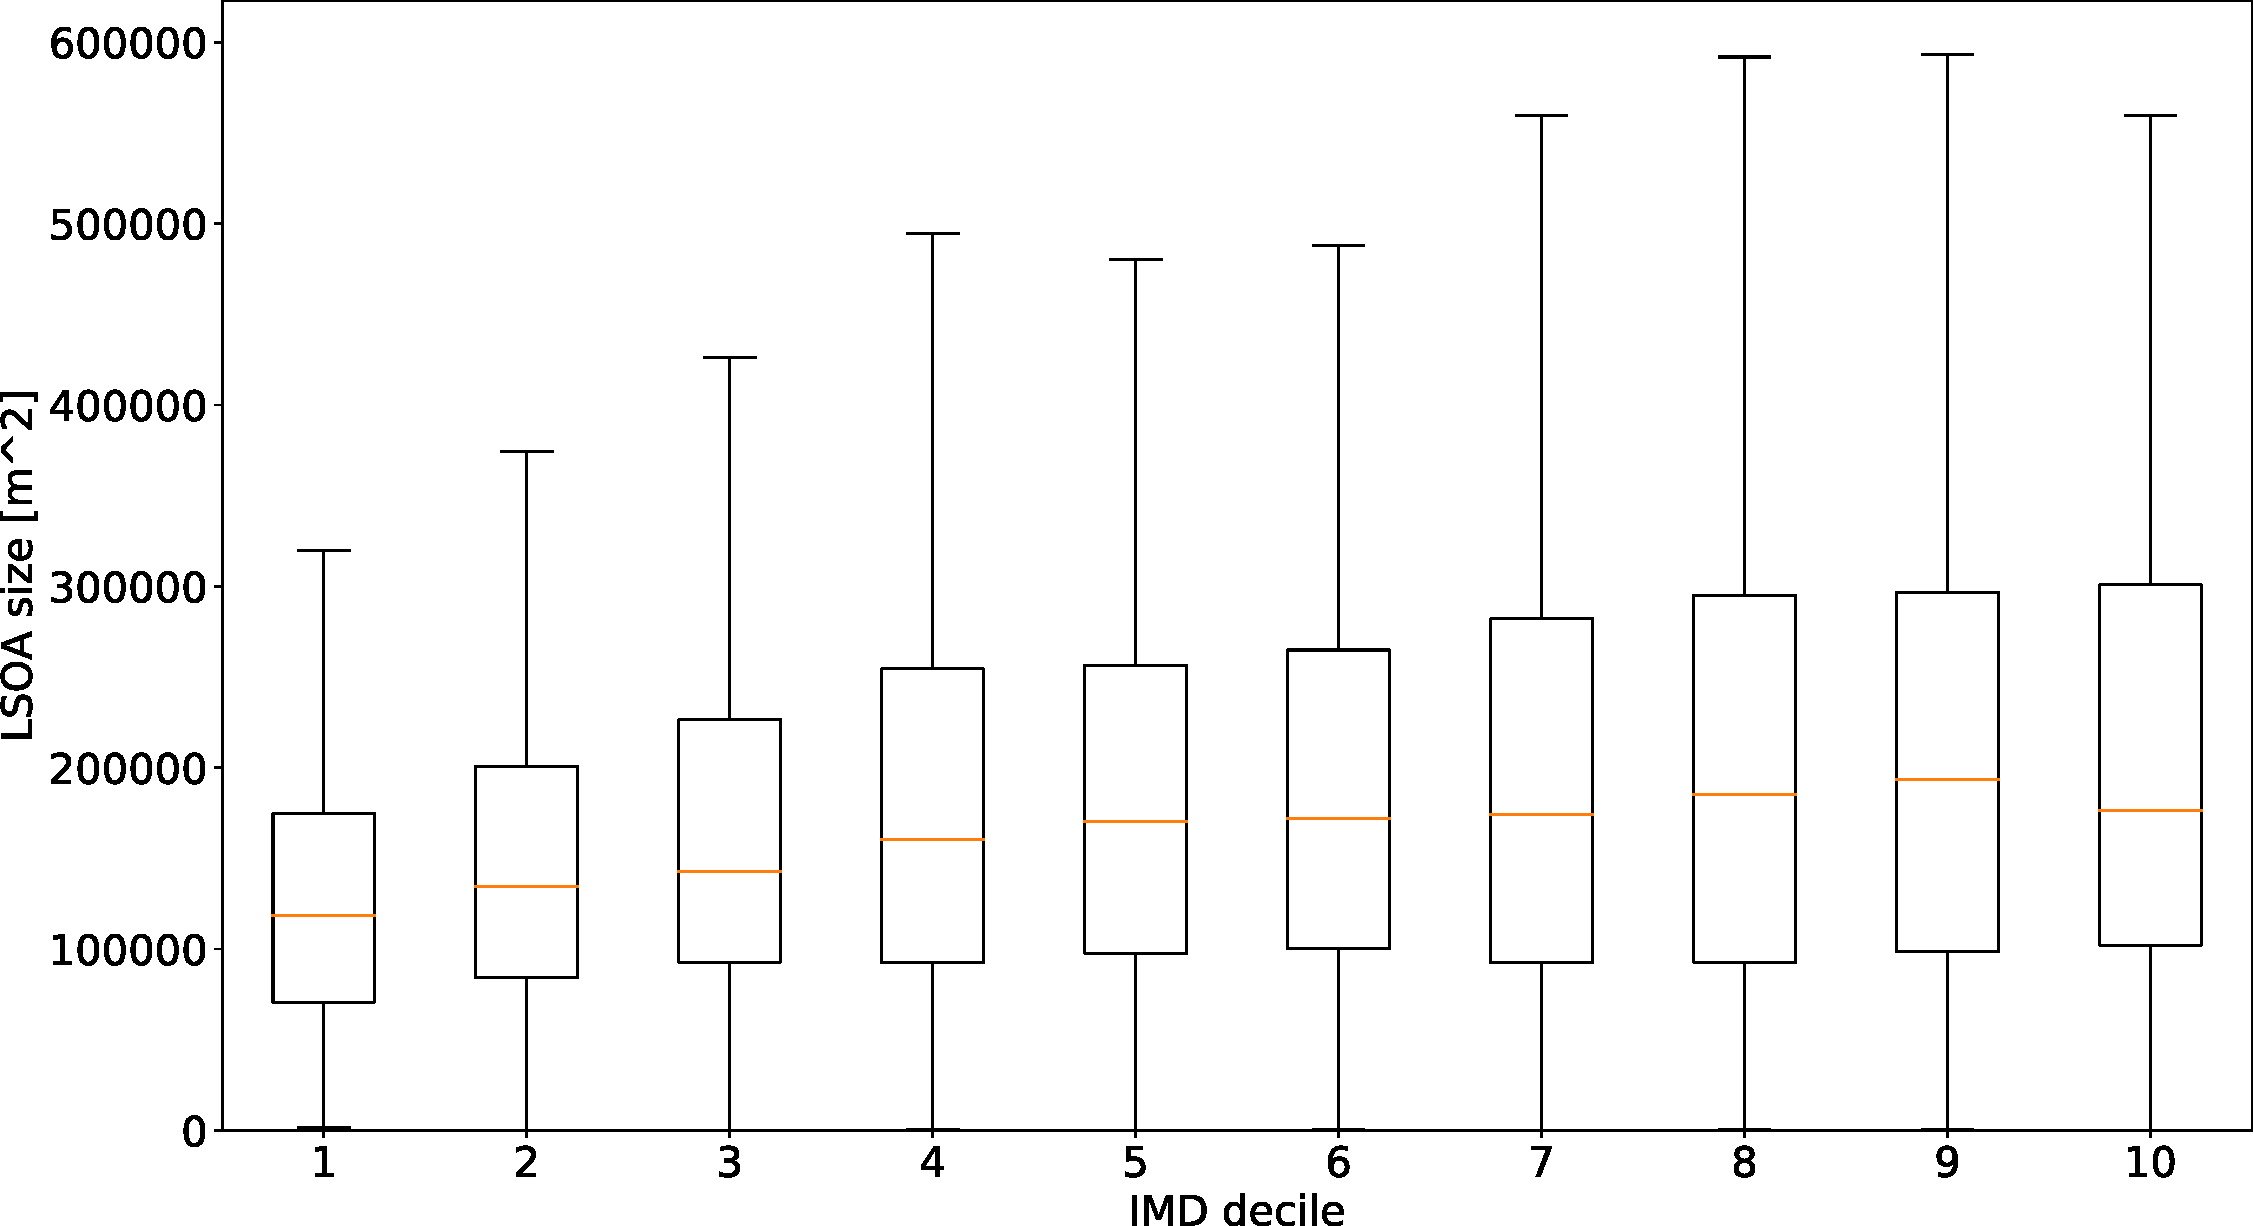
\includegraphics[width=0.7\linewidth]{LSOA_size_IMD_decile.pdf}
	\caption{\textit{LSOA size per IMD}}
	\label{fig:LSOA_IMD_size}
\end{figure}

\begin{figure}
	\centering
	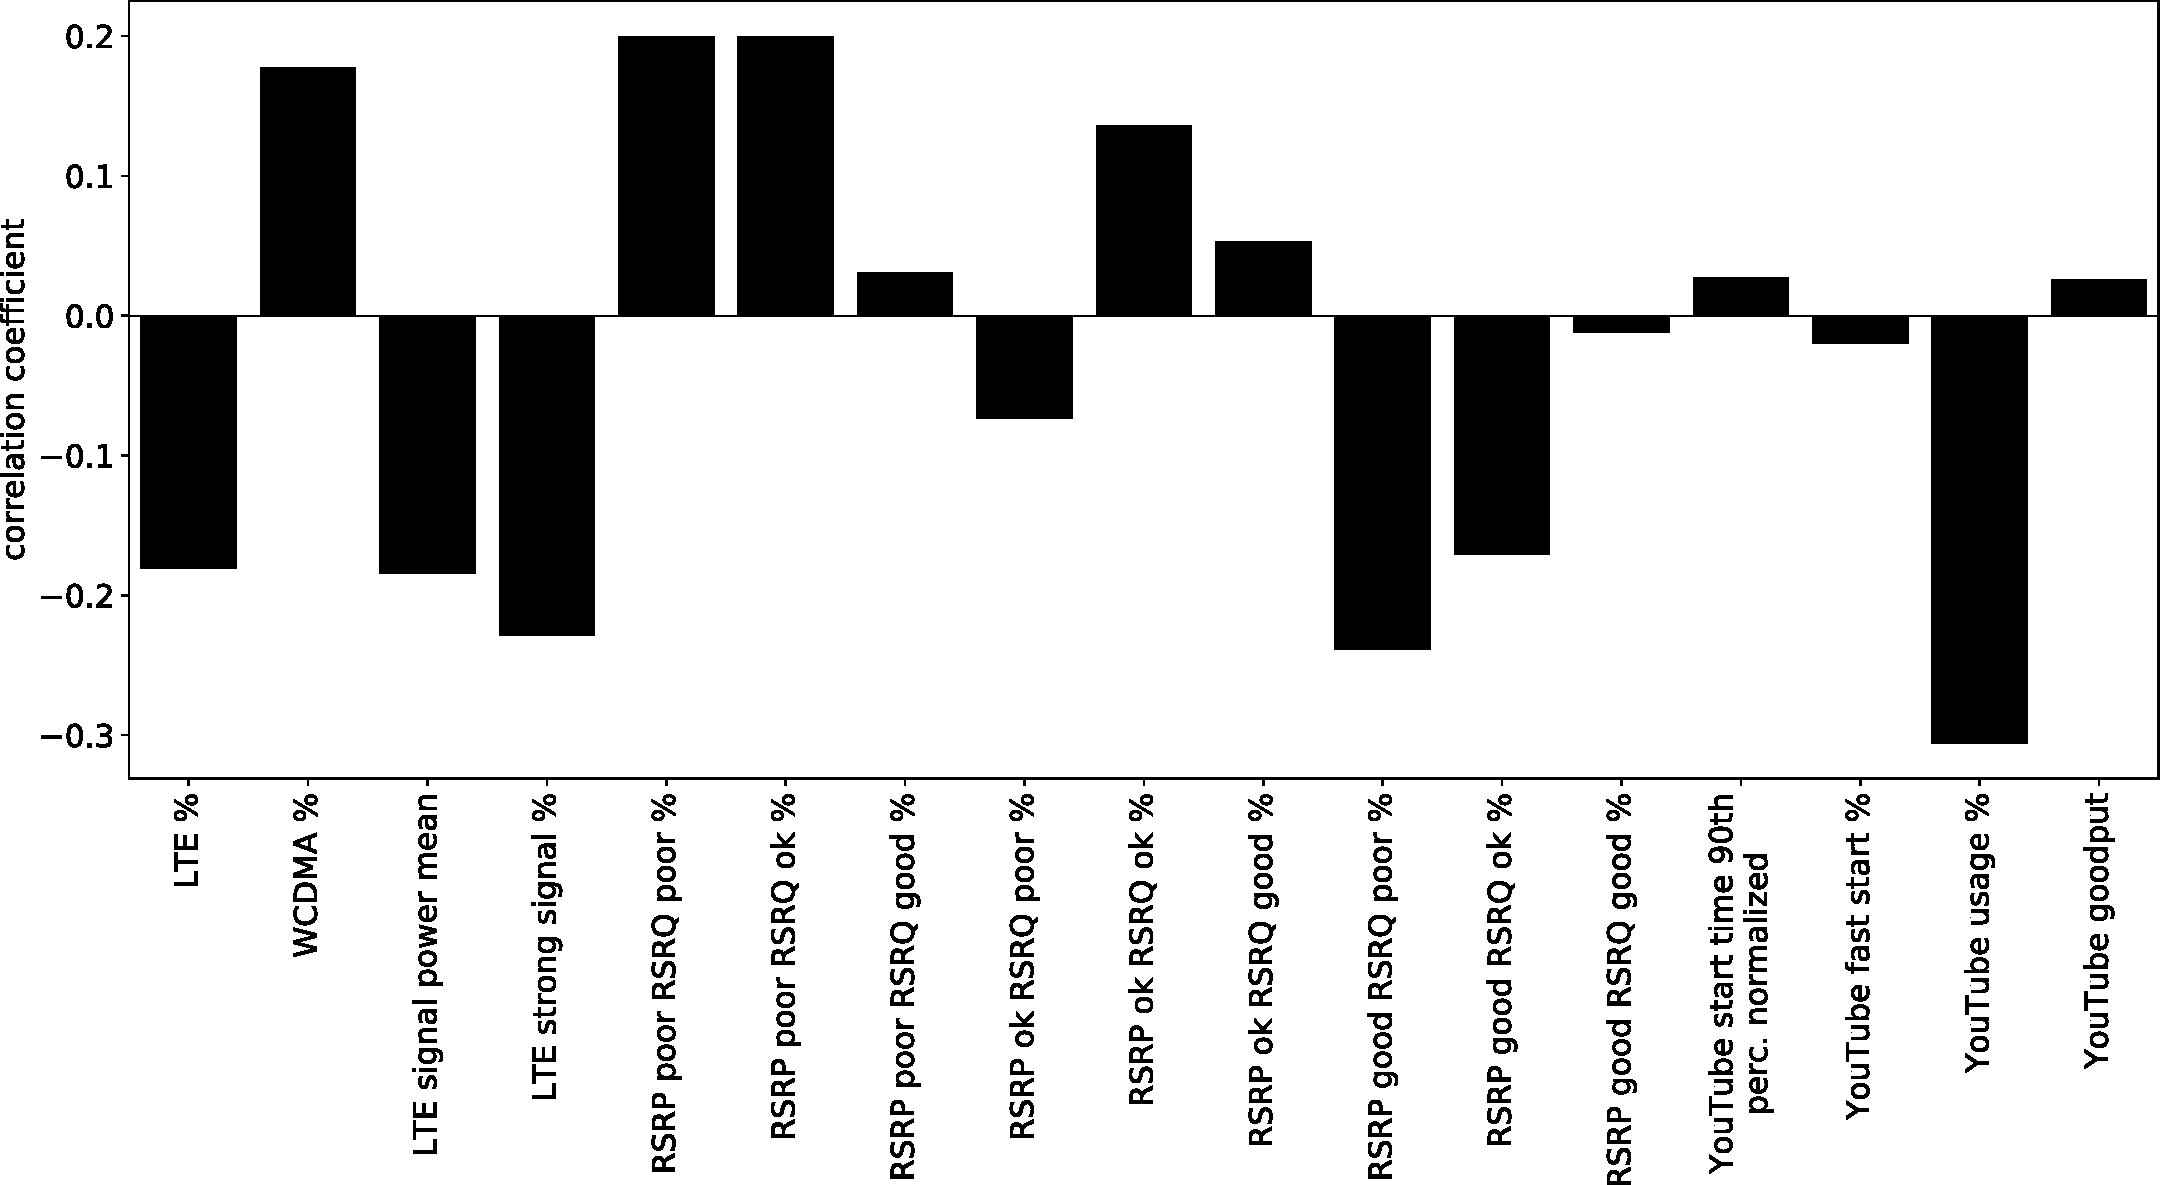
\includegraphics[width=\linewidth]{google_5_week_metrics_correlation_with_IMD_decile_subset.pdf}
	\caption{\textit{Google metrics correlation with IMD decile.}}
	\label{fig:google_metrics_correlation_with_imd_decile}
\end{figure}

\begin{figure}
	\centering
	\begin{subfigure}[b]{0.37	\linewidth}
		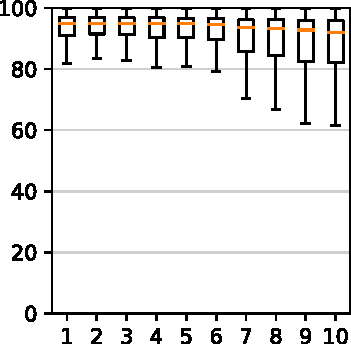
\includegraphics[width=\linewidth,keepaspectratio]{signal_metrics/1_google_signal_features_box_plot_LTE.pdf}
		\caption{\scriptsize{LTE \%}}
	\end{subfigure}
	\hspace{0.5cm}
	\begin{subfigure}[b]{0.37	\linewidth}
		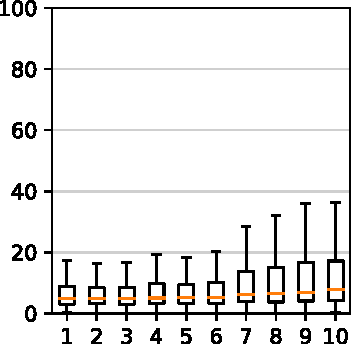
\includegraphics[width=\linewidth,keepaspectratio]{signal_metrics/2_google_signal_features_box_plot_WCDMA.pdf}
		\caption{\scriptsize{WCDMA \%}}
	\end{subfigure}	
	\begin{subfigure}[b]{0.37	\linewidth}
		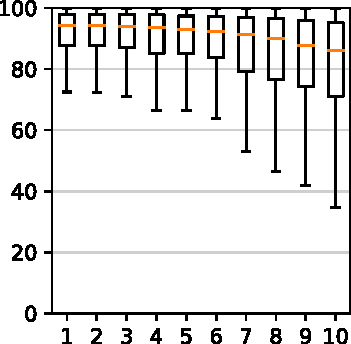
\includegraphics[width=\linewidth,keepaspectratio]{signal_metrics/3_google_signal_features_box_plot_LTE_strong_signal.pdf}
		\caption{\scriptsize{LTE strong signal \%}}
	\end{subfigure}
	\begin{subfigure}[b]{0.45	\linewidth}
		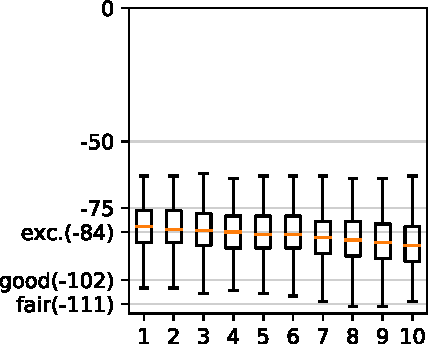
\includegraphics[width=\linewidth,keepaspectratio]{signal_metrics/4_google_signal_features_box_plot_LTE_signal_power_mean[dBm].pdf}
		\caption{\scriptsize{LTE signal power [dBm]}}
	\end{subfigure}
\caption{\textit{Google signal metrics.}}
\label{fig:google_signal_metrics}
\end{figure}

\begin{figure}
\centering
	\begin{subfigure}[b]{0.3	\linewidth}
		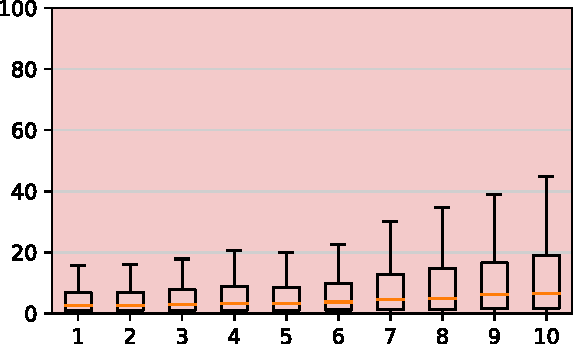
\includegraphics[width=\linewidth,keepaspectratio]{RSRPnRSRQ_metrics/1_google_RSRPnRSRQ_box_RSRPpoorRSRQpoor.pdf}
		\caption{\tiny{RSRP poor RSRQ poor \%}}
	\end{subfigure}
	\begin{subfigure}[b]{0.3	\linewidth}
		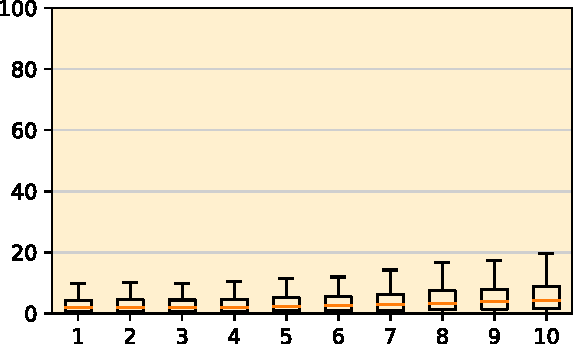
\includegraphics[width=\linewidth,keepaspectratio]{RSRPnRSRQ_metrics/2_google_RSRPnRSRQ_box_RSRPpoorRSRQok.pdf}
		\caption{\tiny{RSRP poor RSRQ ok \%}}
	\end{subfigure}
	\begin{subfigure}[b]{0.3	\linewidth}
		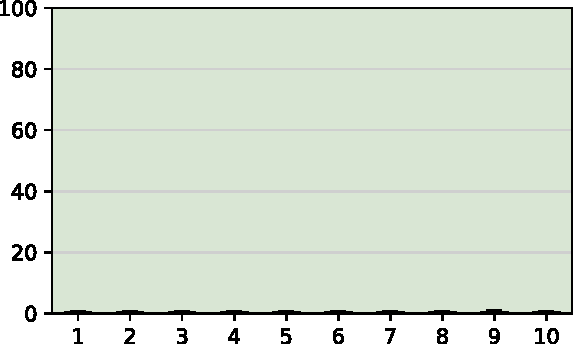
\includegraphics[width=\linewidth,keepaspectratio]{RSRPnRSRQ_metrics/3_google_RSRPnRSRQ_box_RSRPpoorRSRQgood.pdf}
		\caption{\tiny{RSRP poor RSRQ good \%}}
	\end{subfigure}
	\begin{subfigure}[b]{0.3	\linewidth}
		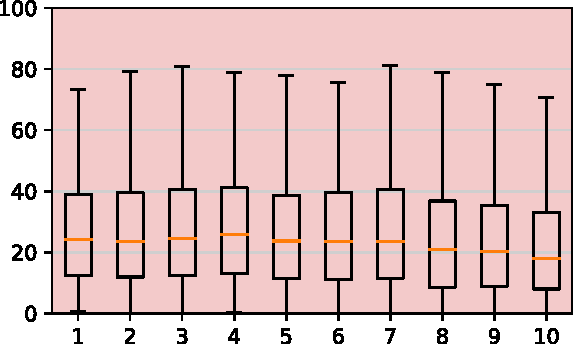
\includegraphics[width=\linewidth,keepaspectratio]{RSRPnRSRQ_metrics/4_google_RSRPnRSRQ_box_RSRPokRSRQpoor.pdf}
		\caption{\tiny{RSRP ok RSRQ poor \%}}
	\end{subfigure}
	\begin{subfigure}[b]{0.3	\linewidth}
		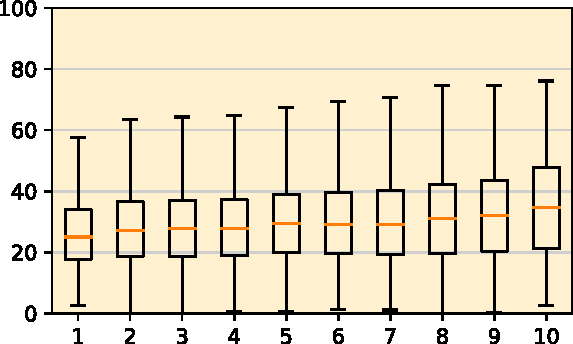
\includegraphics[width=\linewidth,keepaspectratio]{RSRPnRSRQ_metrics/5_google_RSRPnRSRQ_box_RSRPokRSRQok.pdf}
		\caption{\tiny{RSRP ok RSRQ ok \%}}
	\end{subfigure}
	\begin{subfigure}[b]{0.3	\linewidth}
		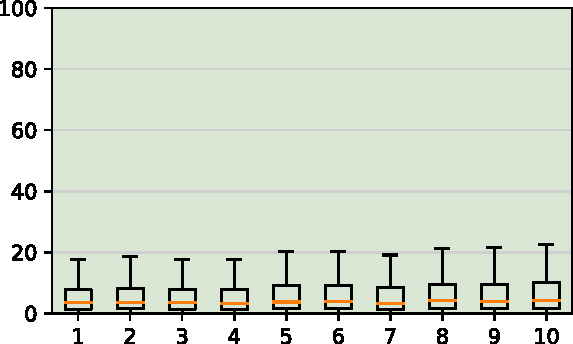
\includegraphics[width=\linewidth,keepaspectratio]{RSRPnRSRQ_metrics/6_google_RSRPnRSRQ_box_RSRPokRSRQgood.pdf}
		\caption{\tiny{RSRP ok RSRQ good \%}}
	\end{subfigure}
	\begin{subfigure}[b]{0.3	\linewidth}
		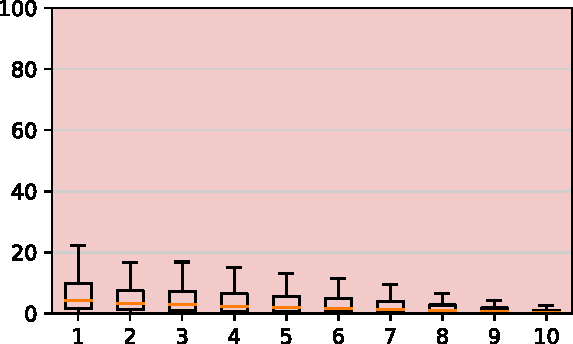
\includegraphics[width=\linewidth,keepaspectratio]{RSRPnRSRQ_metrics/7_google_RSRPnRSRQ_box_RSRPgoodRSRQpoor.pdf}
		\caption{\tiny{RSRP good RSRQ poor \%}}
	\end{subfigure}
	\begin{subfigure}[b]{0.3	\linewidth}
		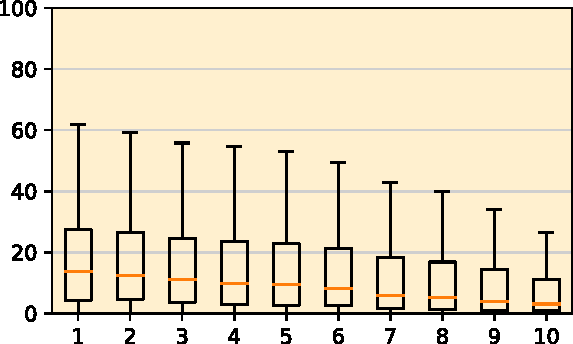
\includegraphics[width=\linewidth,keepaspectratio]{RSRPnRSRQ_metrics/8_google_RSRPnRSRQ_box_RSRPgoodRSRQok.pdf}
		\caption{\tiny{RSRP good RSRQ ok \%}}
	\end{subfigure}
	\begin{subfigure}[b]{0.3	\linewidth}
		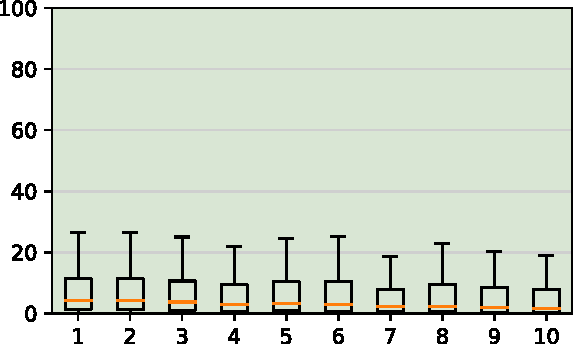
\includegraphics[width=\linewidth,keepaspectratio]{RSRPnRSRQ_metrics/9_google_RSRPnRSRQ_box_RSRPgoodRSRQgood.pdf}
		\caption{\tiny{RSRP good RSRQ good \%}}
	\end{subfigure}
\caption{\textit{Google RSRP/RSRQ intersectional metrics.}}
\label{fig:google_RSRPnRSRQ_metrics}
\end{figure}

\begin{figure}
\centering
	\begin{subfigure}[b]{0.4	\linewidth}
		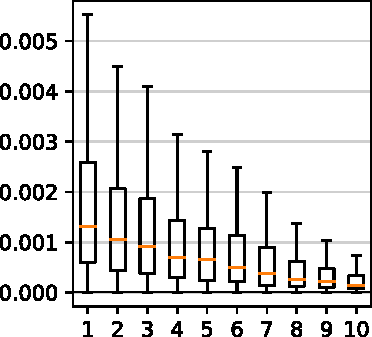
\includegraphics[width=\linewidth,keepaspectratio]{youtube_metrics/1_google_youtube_features_box_plot_youtube_usage.pdf}
		\caption{\scriptsize{YouTube usage \%\\\hspace{\textwidth}}}
	\end{subfigure}
	\begin{subfigure}[b]{0.45	\linewidth}
		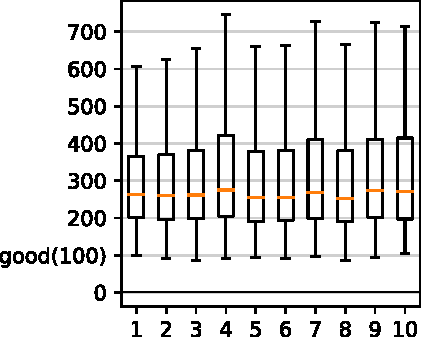
\includegraphics[width=\linewidth,keepaspectratio]{youtube_metrics/3_google_youtube_features_box_plot_youtube_start_time_90thpercentile_normalized[ms].pdf}
		\caption{\scriptsize{YouTube start time 90th perc. normalized [ms]}}
	\end{subfigure}
	
	\hspace{0.1cm}
	\begin{subfigure}[b]{0.37	\linewidth}
		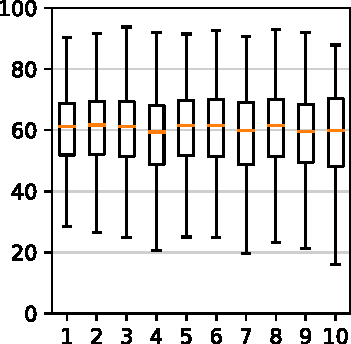
\includegraphics[width=\linewidth,keepaspectratio]{youtube_metrics/4_google_youtube_features_box_plot_youtube_fast_start.pdf}
		\caption{\scriptsize{YouTube fast start \%}}
	\end{subfigure}
	\begin{subfigure}[b]{0.45	\linewidth}
		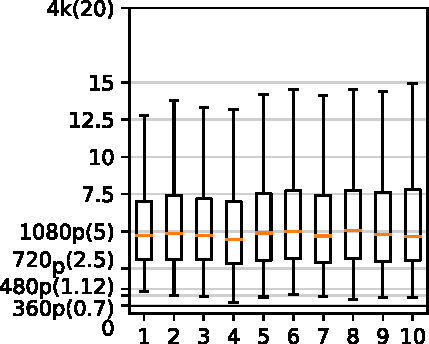
\includegraphics[width=\linewidth,keepaspectratio]{youtube_metrics/5_google_youtube_features_box_plot_youtube_goodput_[Mbps].pdf}
		\caption{\scriptsize{YouTube goodput [Mbps]}}
		\label{fig:google_youtube_metrics_goodput}
	\end{subfigure}
\caption{\textit{Google YouTube metrics.}}
\label{fig:google_youtube_metrics}
\end{figure}

\subsection{Outliers analysis}

We analysed the outliers, i.e. fliers in the boxplots, by visualizing them on a map and putting them into context of their neighborhood and IMD value for give LSOAs, Fig.~\ref{fig:google_metrics_outliers}.
[TBD by Pavol - maybe change the visualization or the description under the maps to make it easier to understand and search for explanation of the outliers]

\begin{figure*}
\centering
	\begin{subfigure}[b]{0.3	\linewidth}
		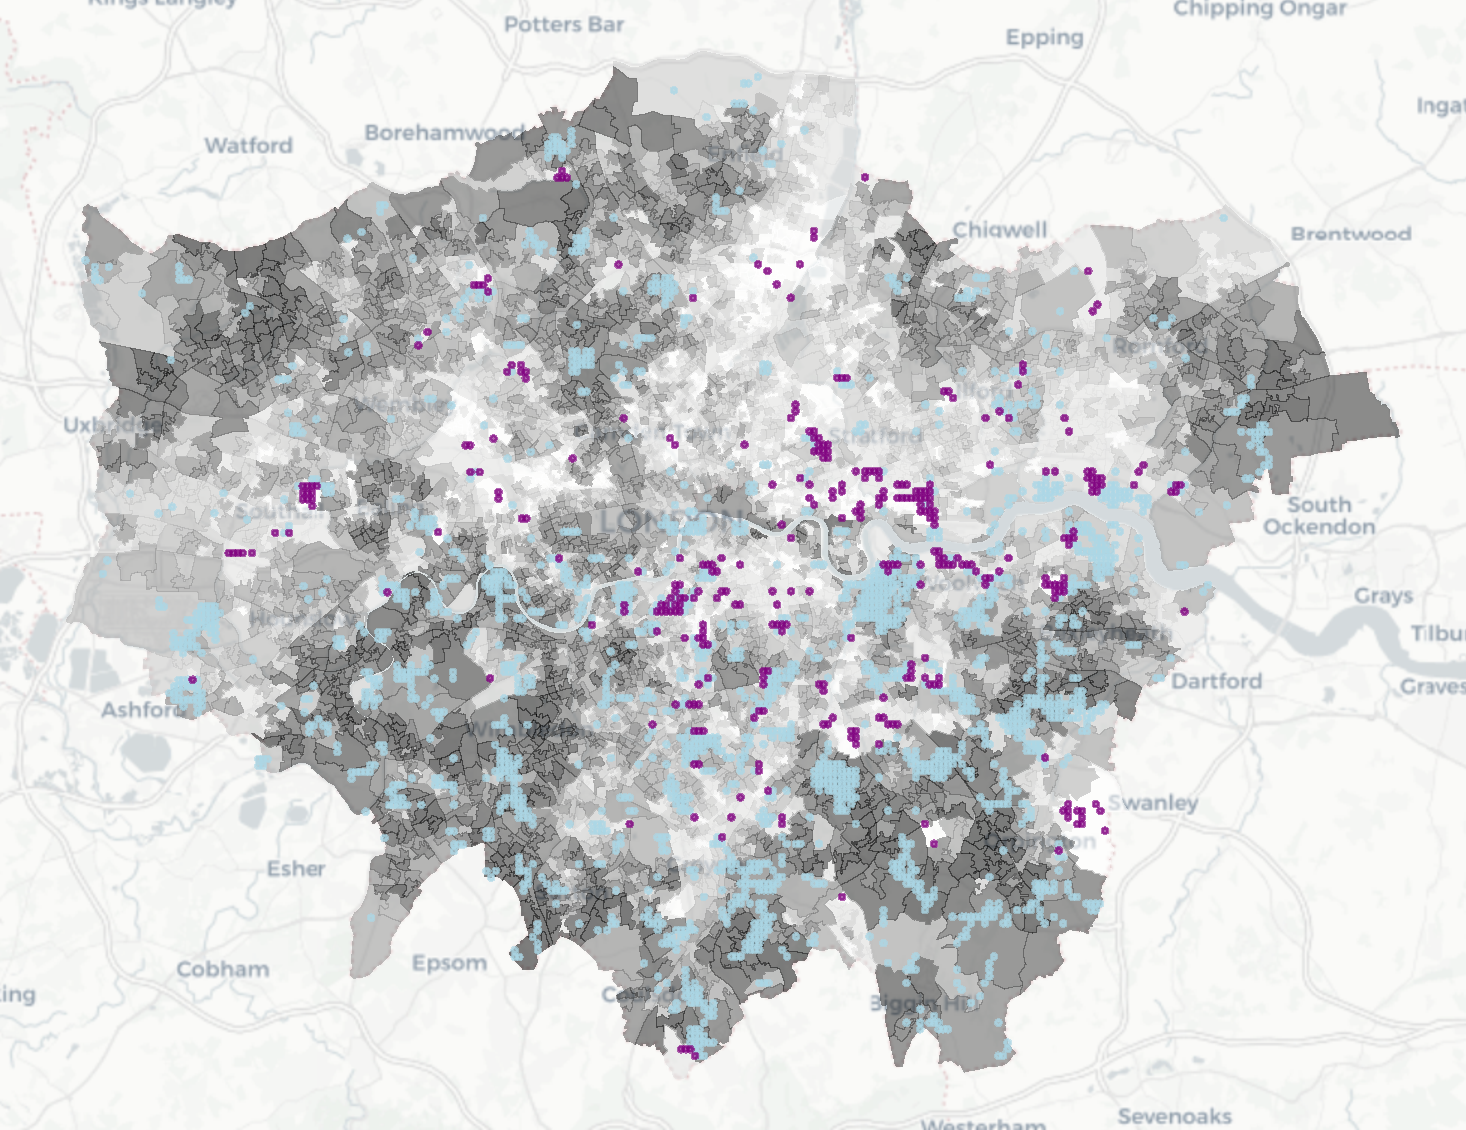
\includegraphics[width=\linewidth,keepaspectratio]{fliers/LTE_lower_fliers_2colors_IMD.pdf}
		\caption{\scriptsize{LTE \% low outliers}}
	\end{subfigure}	
	\begin{subfigure}[b]{0.3	\linewidth}
		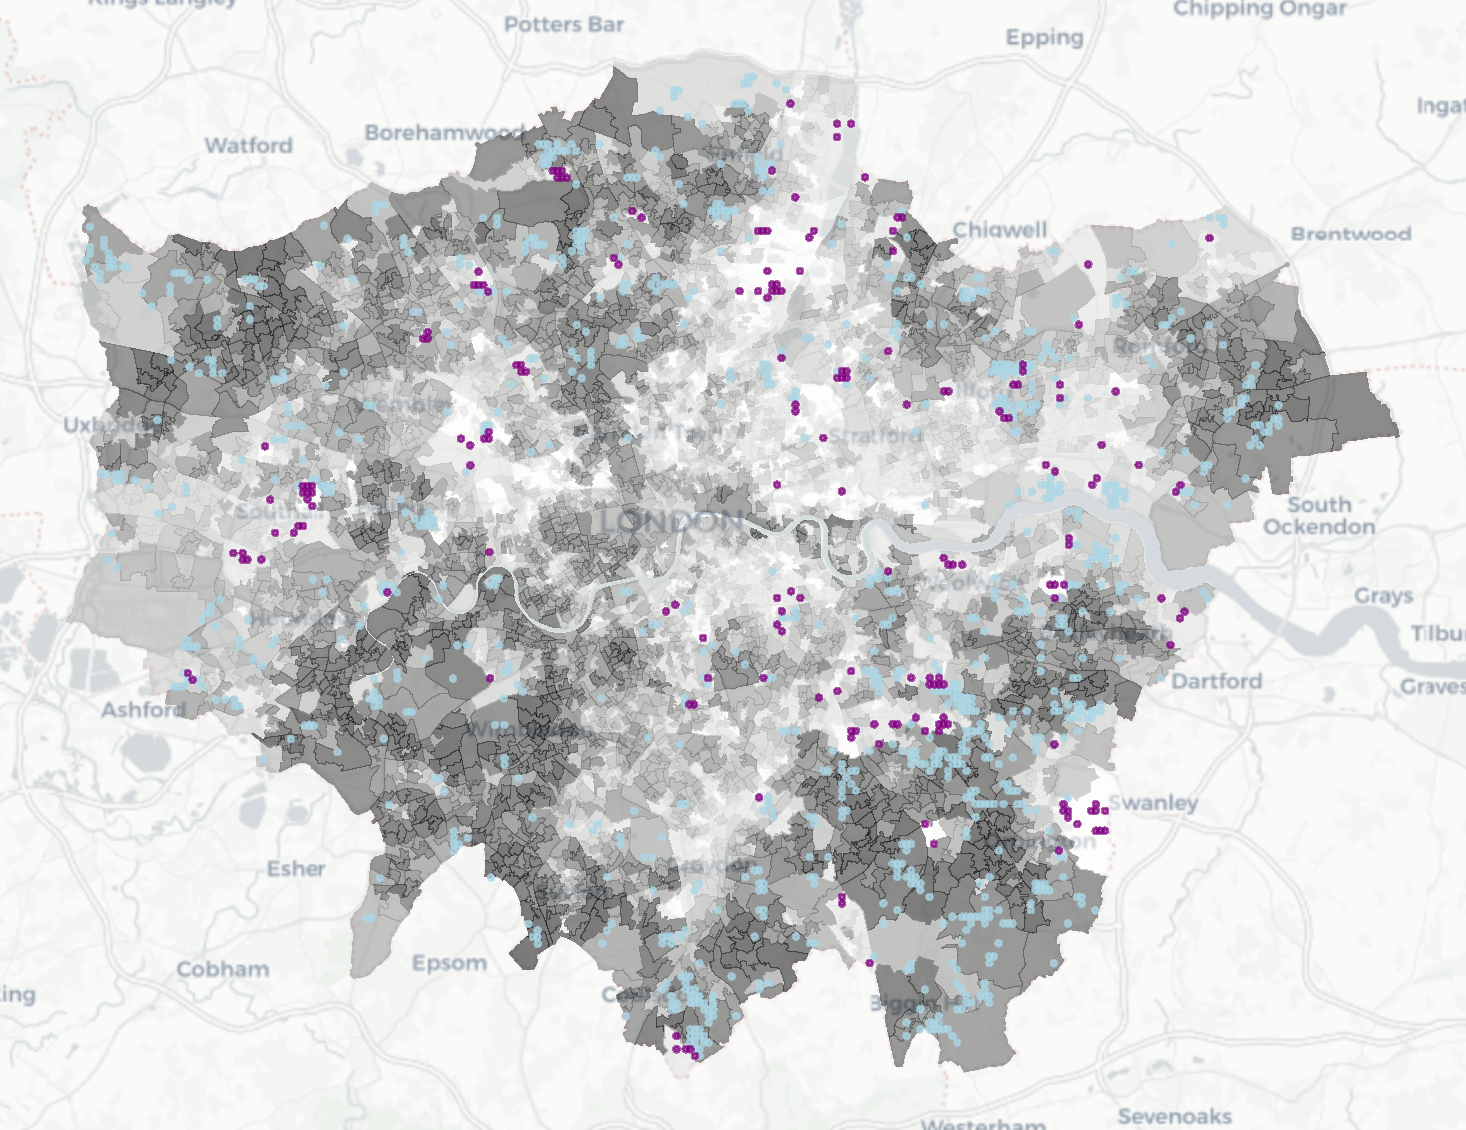
\includegraphics[width=\linewidth,keepaspectratio]{fliers/LTE_strong_signal_lower_fliers_2colors_IMD.pdf}
		\caption{\scriptsize{LTE strong signal \% low outliers}}
	\end{subfigure}
	\begin{subfigure}[b]{0.3	\linewidth}
		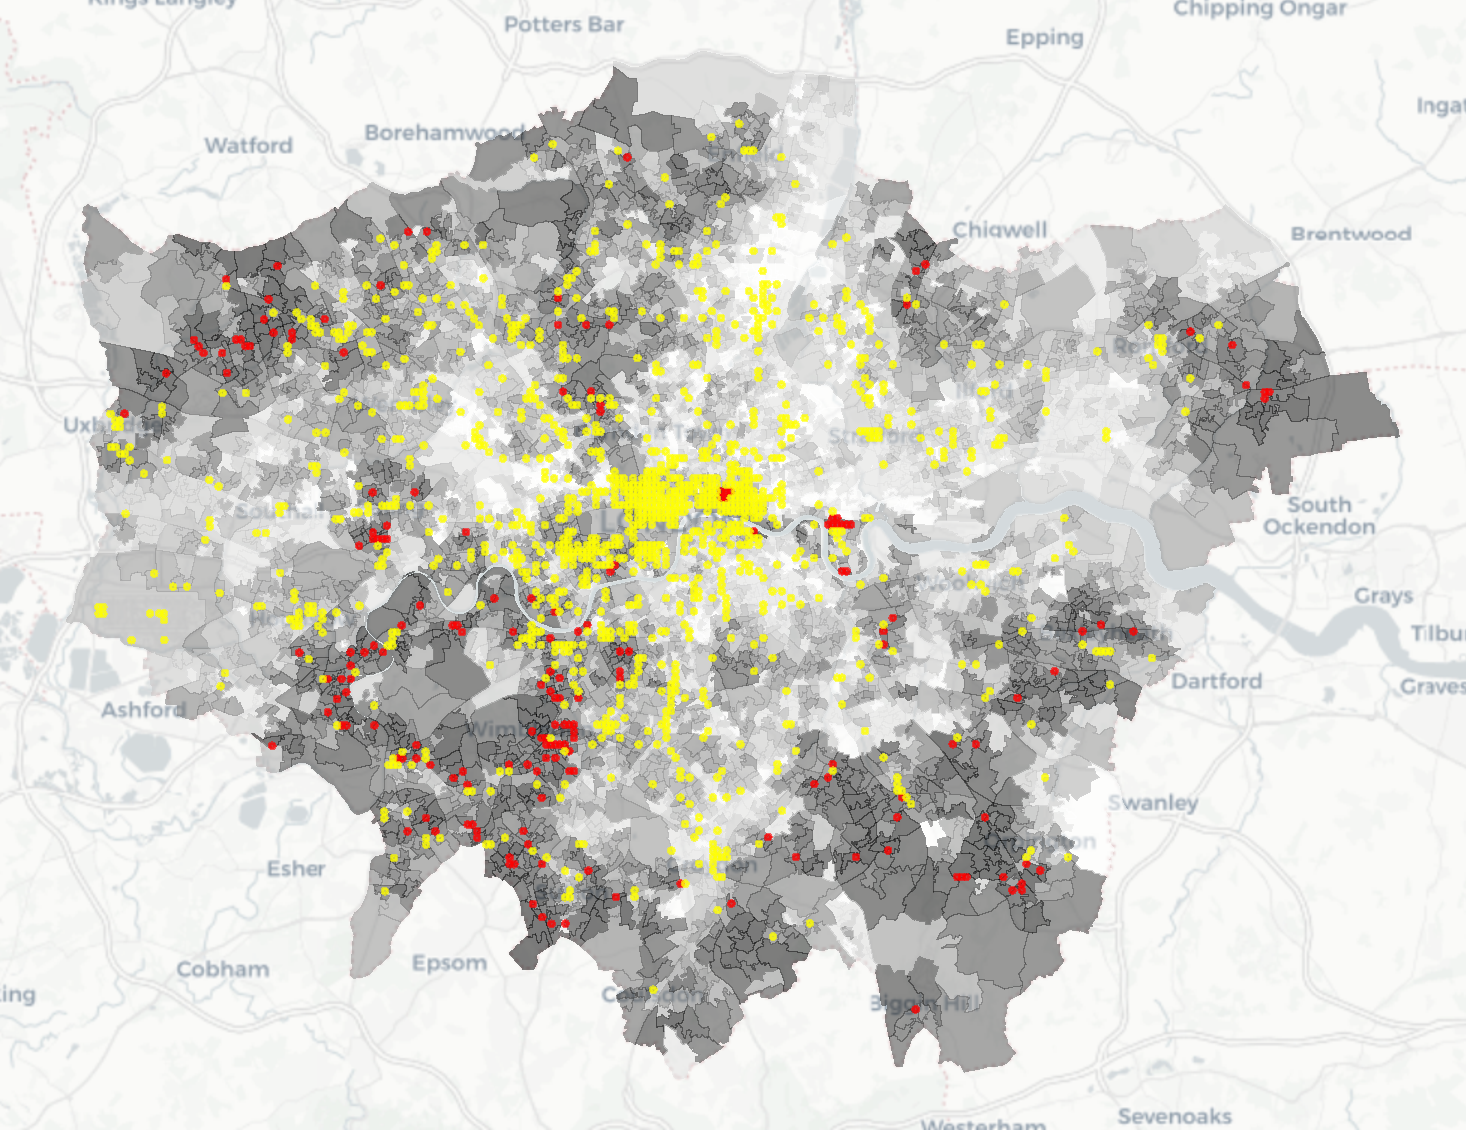
\includegraphics[width=\linewidth,keepaspectratio]{fliers/youtube_usage_higher_fliers_2colors_IMD.pdf}
		\caption{\scriptsize{YouTube usage \% high outliers}}
	\end{subfigure}
	\begin{subfigure}[b]{0.3	\linewidth}
		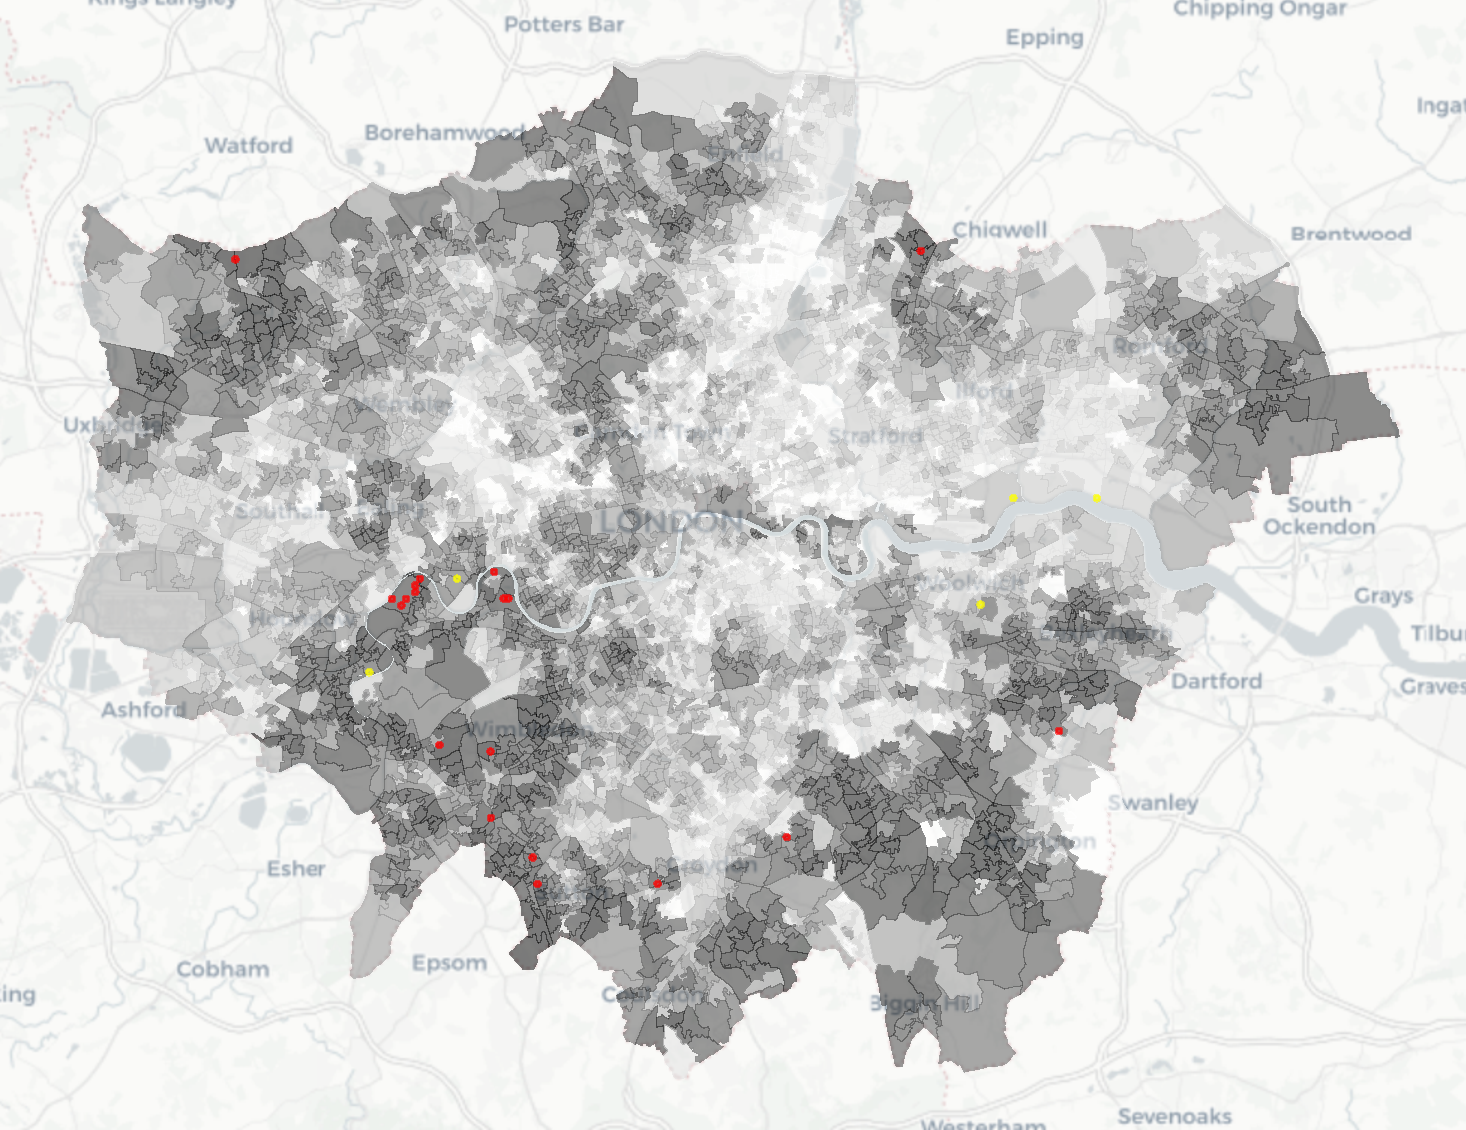
\includegraphics[width=\linewidth,keepaspectratio]{fliers/RSRPokRSRQpoor_higher_fliers_2colors_IMD.pdf}
		\caption{\scriptsize{RSRP ok RSRQ poor \% high outliers}}
	\end{subfigure}	
	\begin{subfigure}[b]{0.3	\linewidth}
		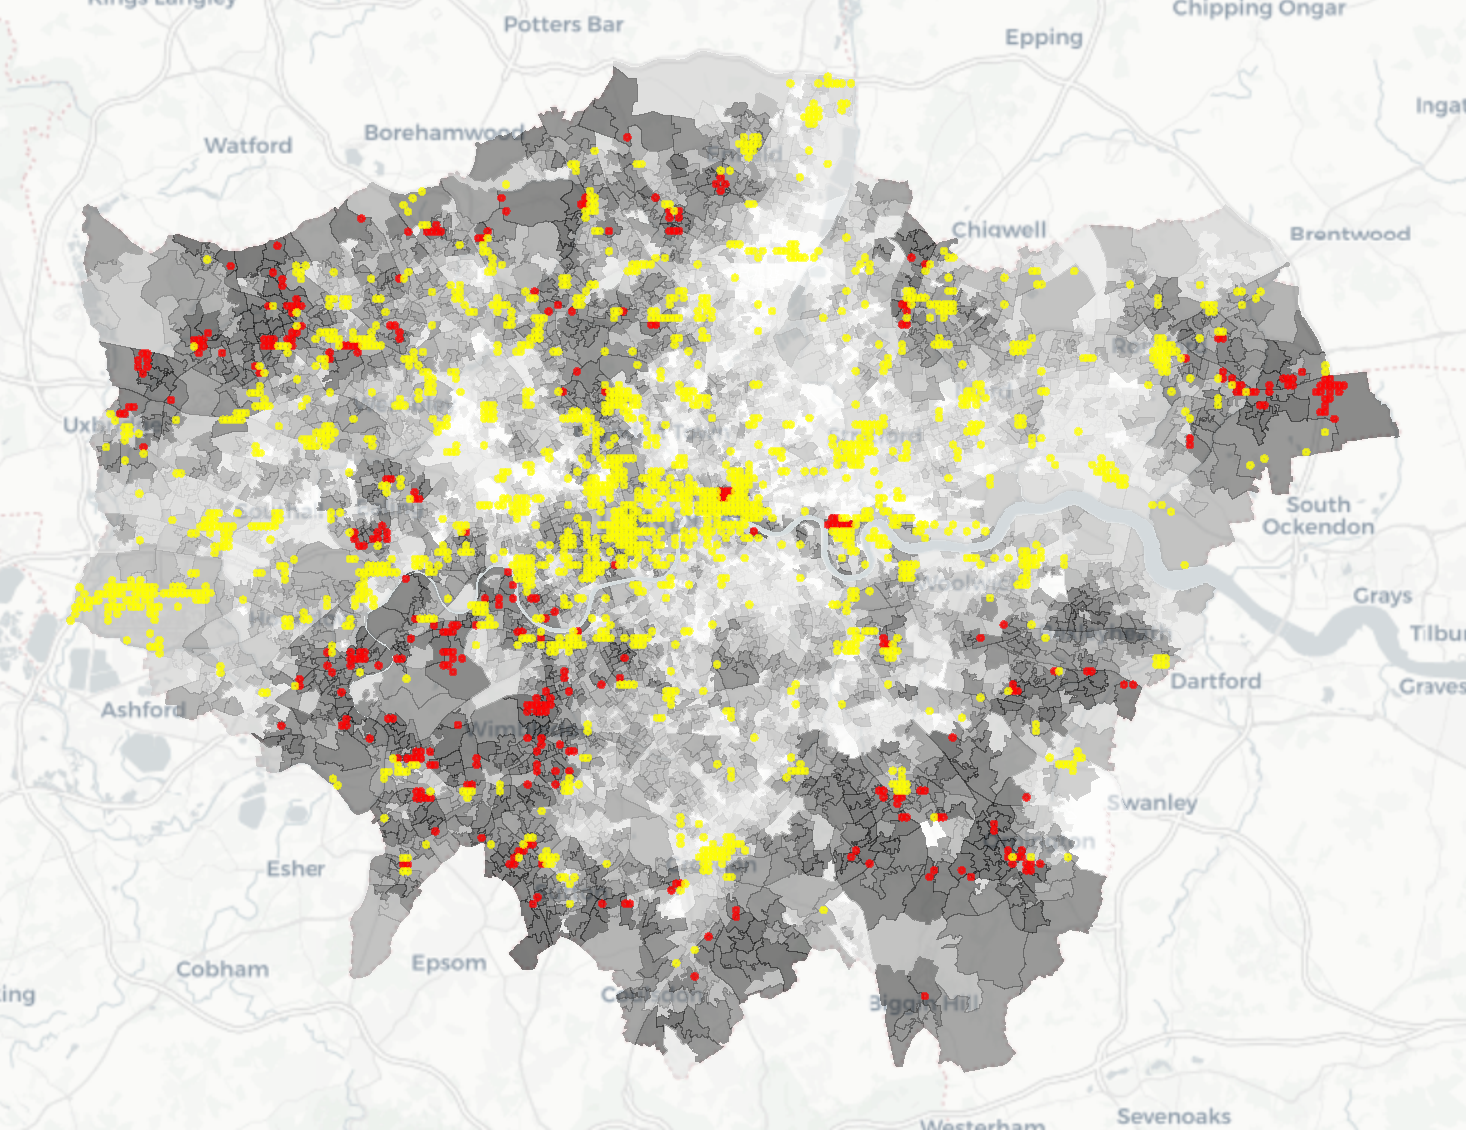
\includegraphics[width=\linewidth,keepaspectratio]{fliers/RSRPgoodRSRQpoor_higher_fliers_2colors_IMD.pdf}
		\caption{\scriptsize{RSRP good RSRQ poor \% high outliers}}
	\end{subfigure}
	\begin{subfigure}[b]{0.3	\linewidth}
		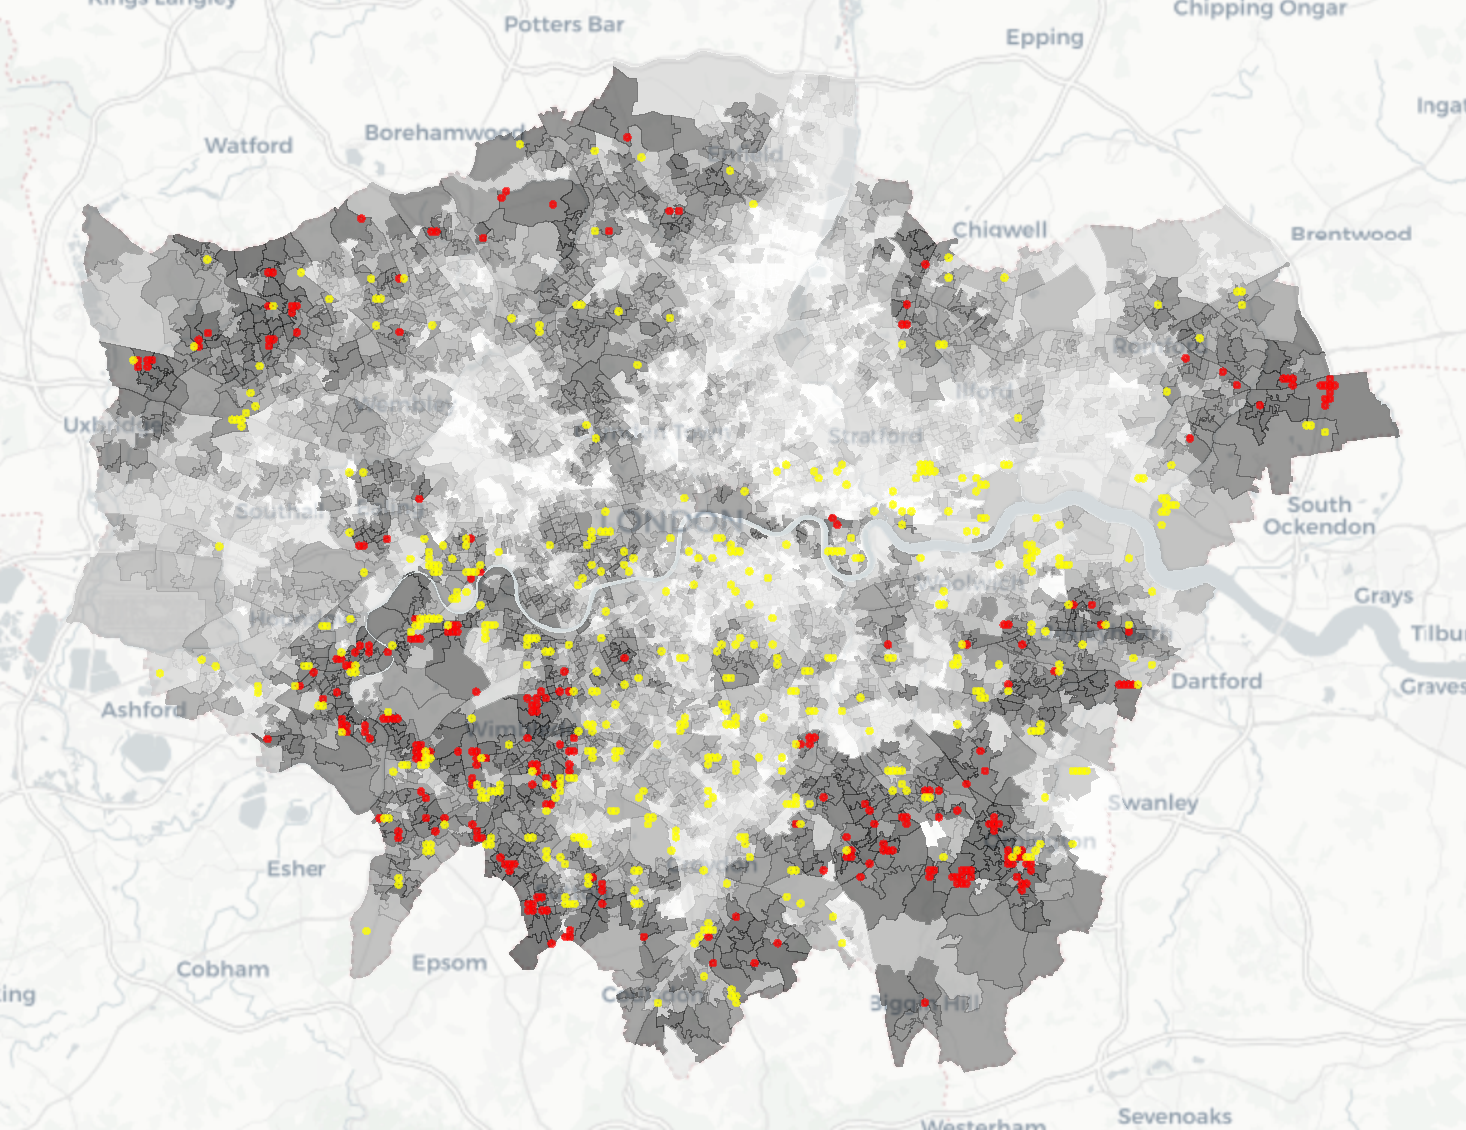
\includegraphics[width=\linewidth,keepaspectratio]{fliers/RSRPgoodRSRQok_higher_fliers_2colors_IMD.pdf}
		\caption{\scriptsize{RSRP good RSRQ ok \% high outliers}}
	\end{subfigure}
\caption{\textit{Google metrics outliers.} We differentiate between high(yellow-red) and low(blue-purple) outliers, i.e. outliers above and below whiskers in the boxplots. Red and purple dots show outliers in the IMD classes where the value of given metric is atypical. Red marks the high outliers in 9-10 IMD Decile LSOAs whereas purple marks low ouliers in 1-2 IMD Decile LSOAs.}
\label{fig:google_metrics_outliers}
\end{figure*}

\subsection{Appendix}
This subsection is just informational and is not usable for the purpose of the conference paper - for the moment at least.
We created a two datasets from LSOA polygon dataset containing IMD decile values. First dataset contains LSOA name and its IDM decile value and seconda contains all neighbors of each LSOA. We fed these dataset to spatial machine learning algorithms in ELKI data mining software to see if there are any LSOA outliers Fig.~\ref{fig:IMD_spatial_outliers}. By LSOA outlier we undestand an LSOA that has IMD value that is significantly locally distinct from its neighbors. The idea is that LSOAs with Google metric outliers might be the ones that are also spatial IMD decile outliers, eg. LSOA with IMD 10 has outliers because it is surrounded by LSOA that have IMD 1.

\begin{figure}
\centering
	\begin{subfigure}[b]{0.45	\linewidth}
		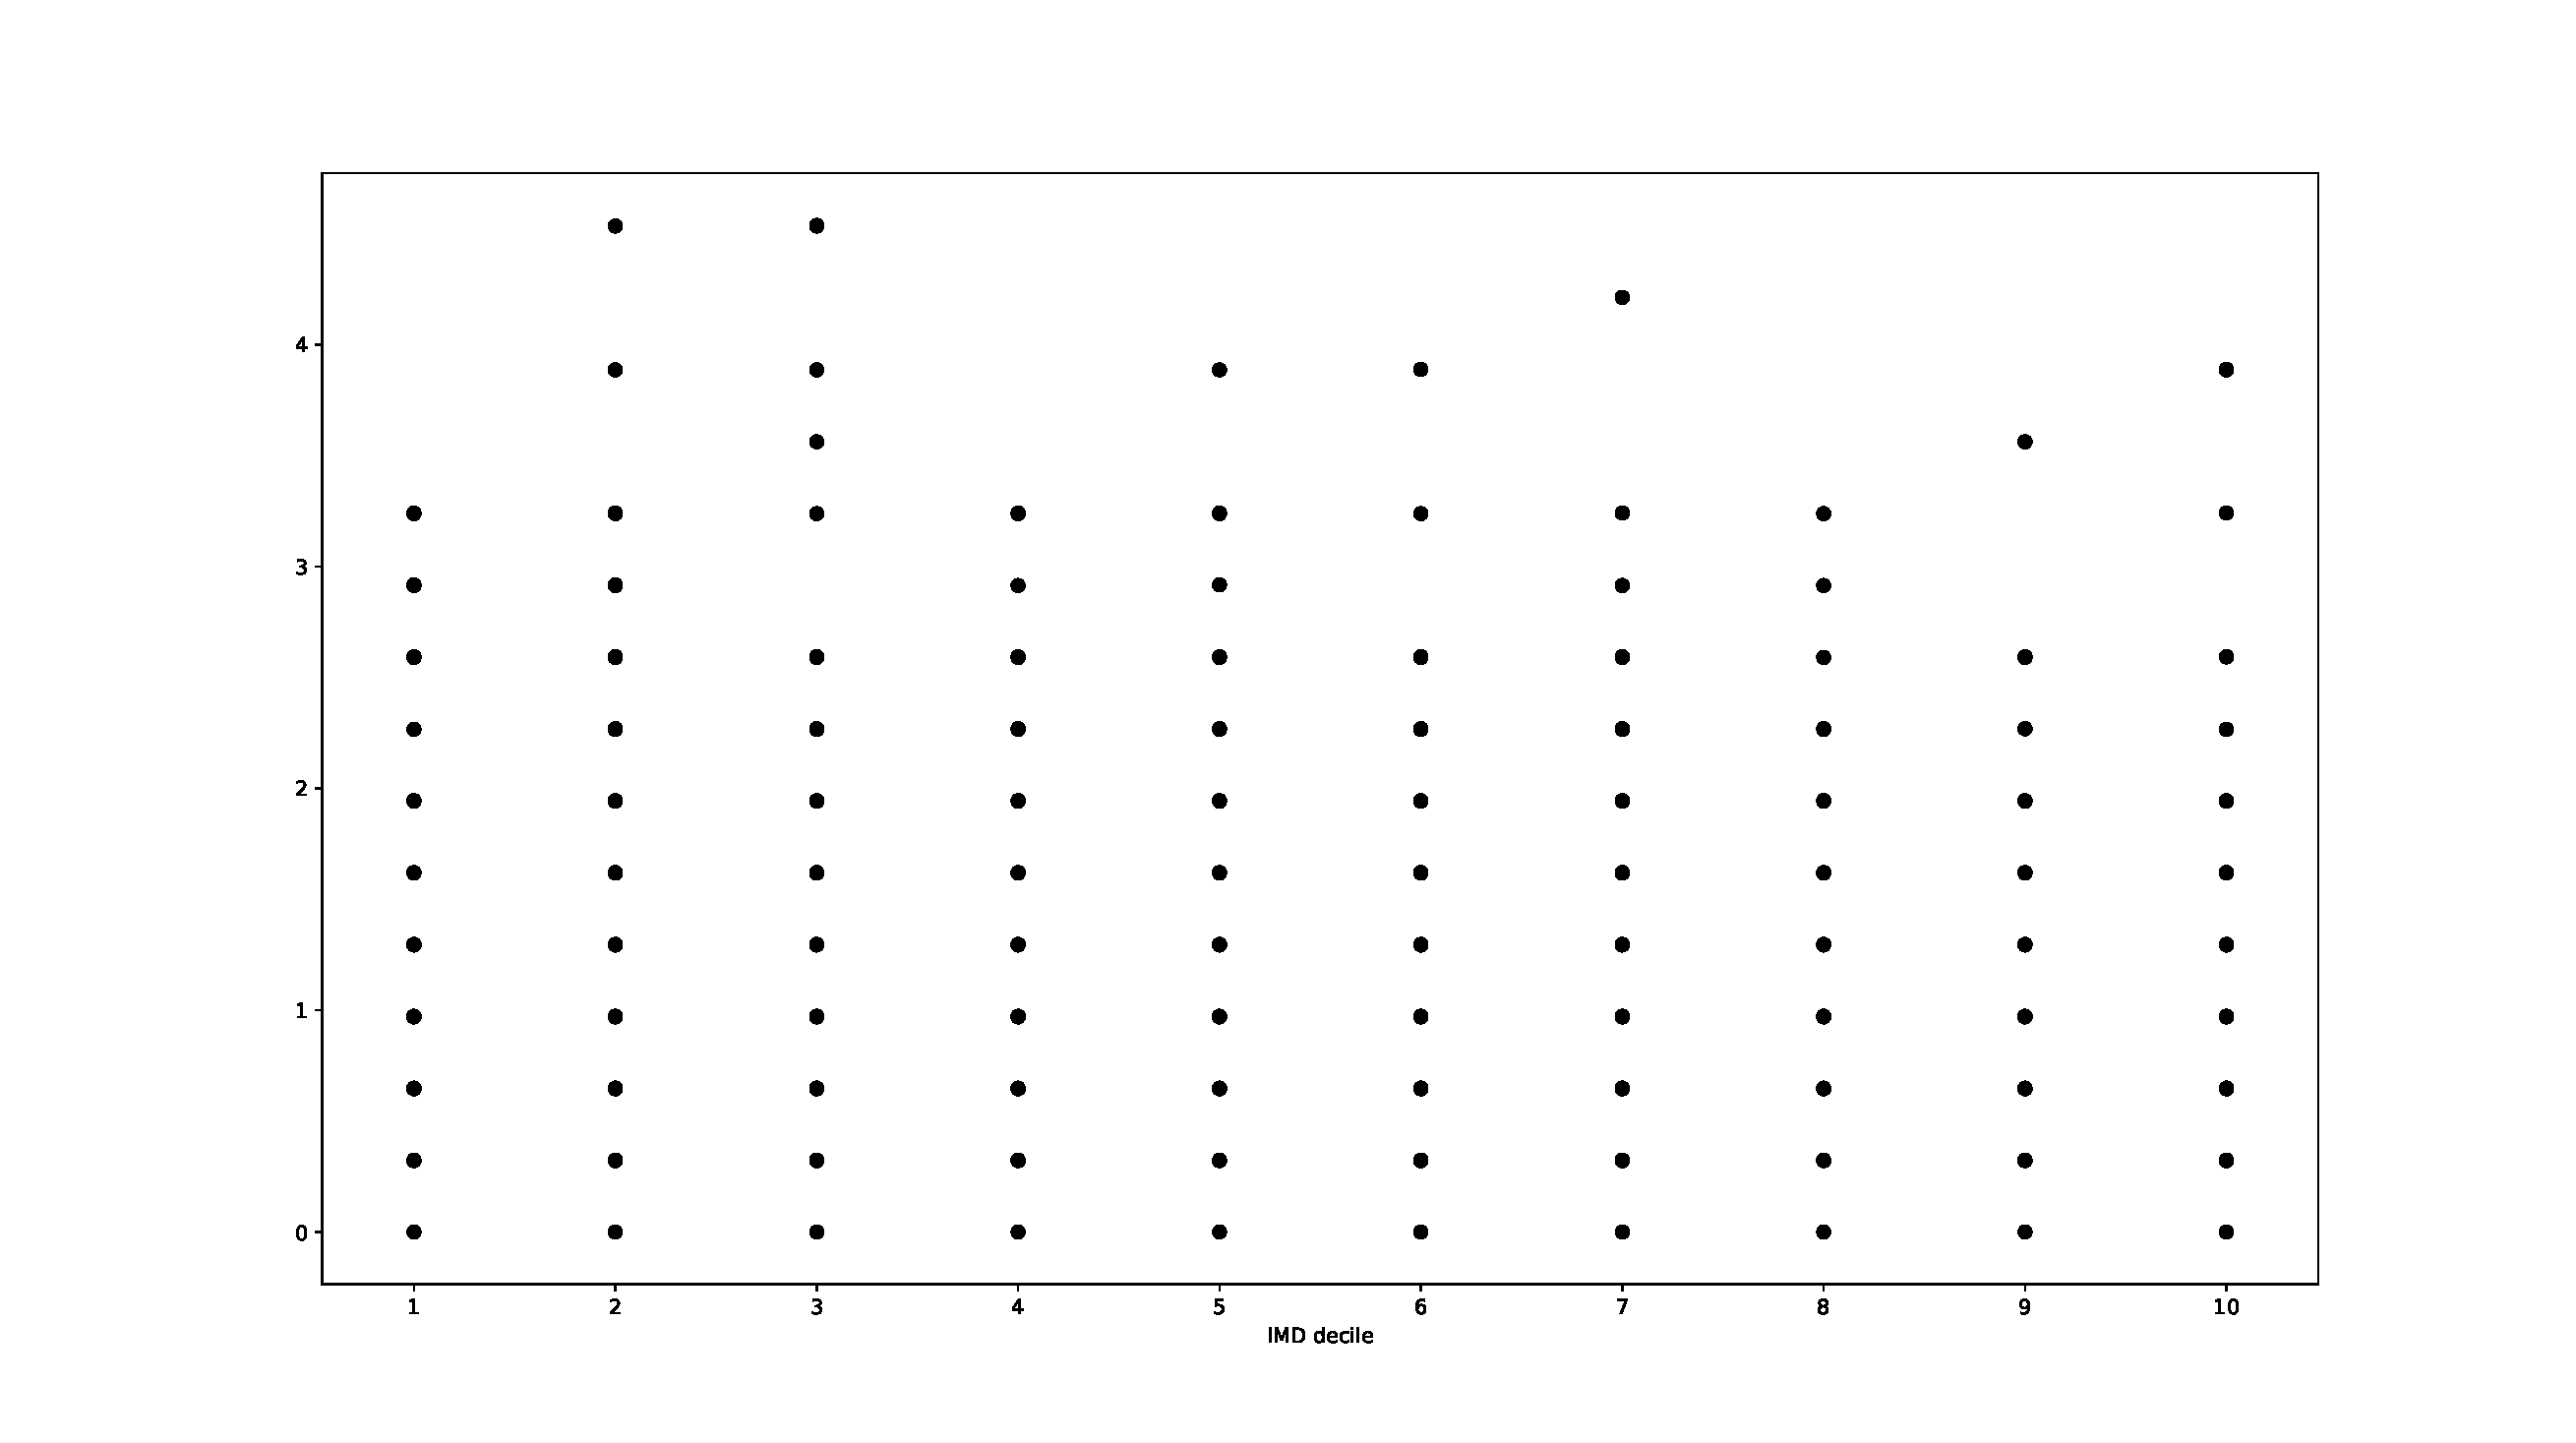
\includegraphics[width=\linewidth,keepaspectratio]{spatial_algorithms/median.pdf}
		\caption{Median}
	\end{subfigure}	
	\begin{subfigure}[b]{0.45	\linewidth}
		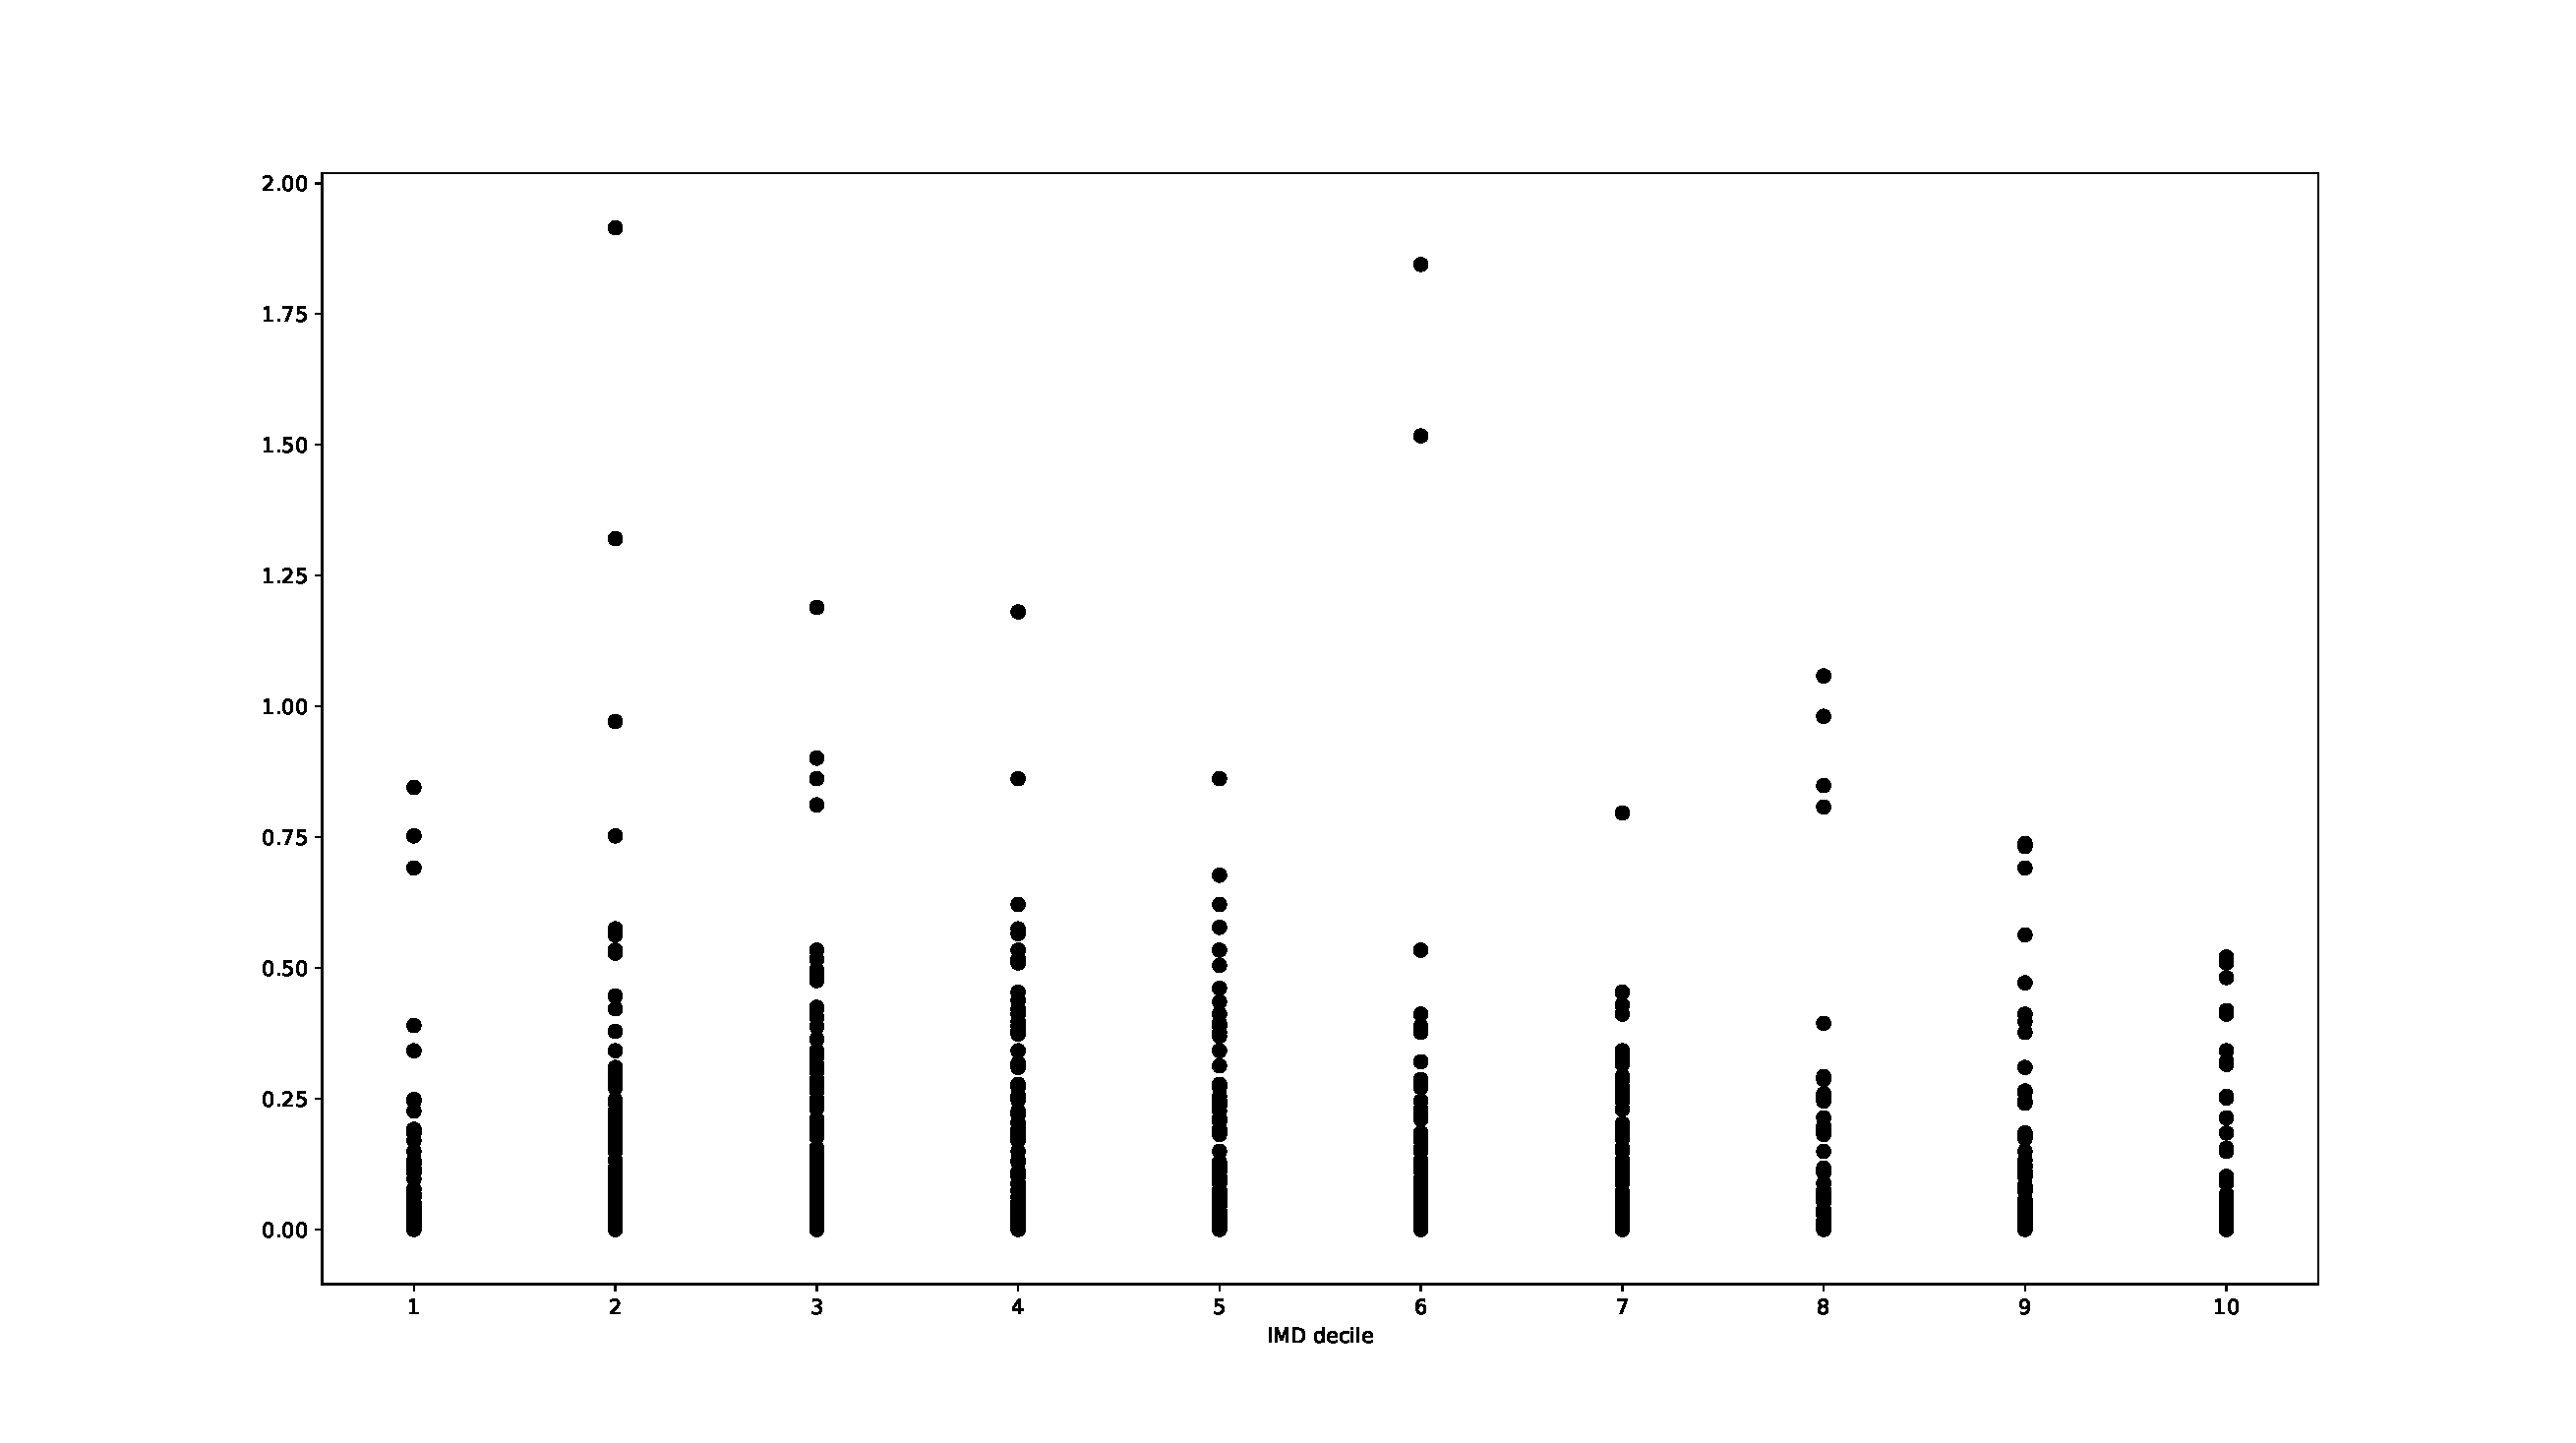
\includegraphics[width=\linewidth,keepaspectratio]{spatial_algorithms/moran_scatter_plot.pdf}
		\caption{Moran scatter plot}
	\end{subfigure}
	\begin{subfigure}[b]{0.45	\linewidth}
		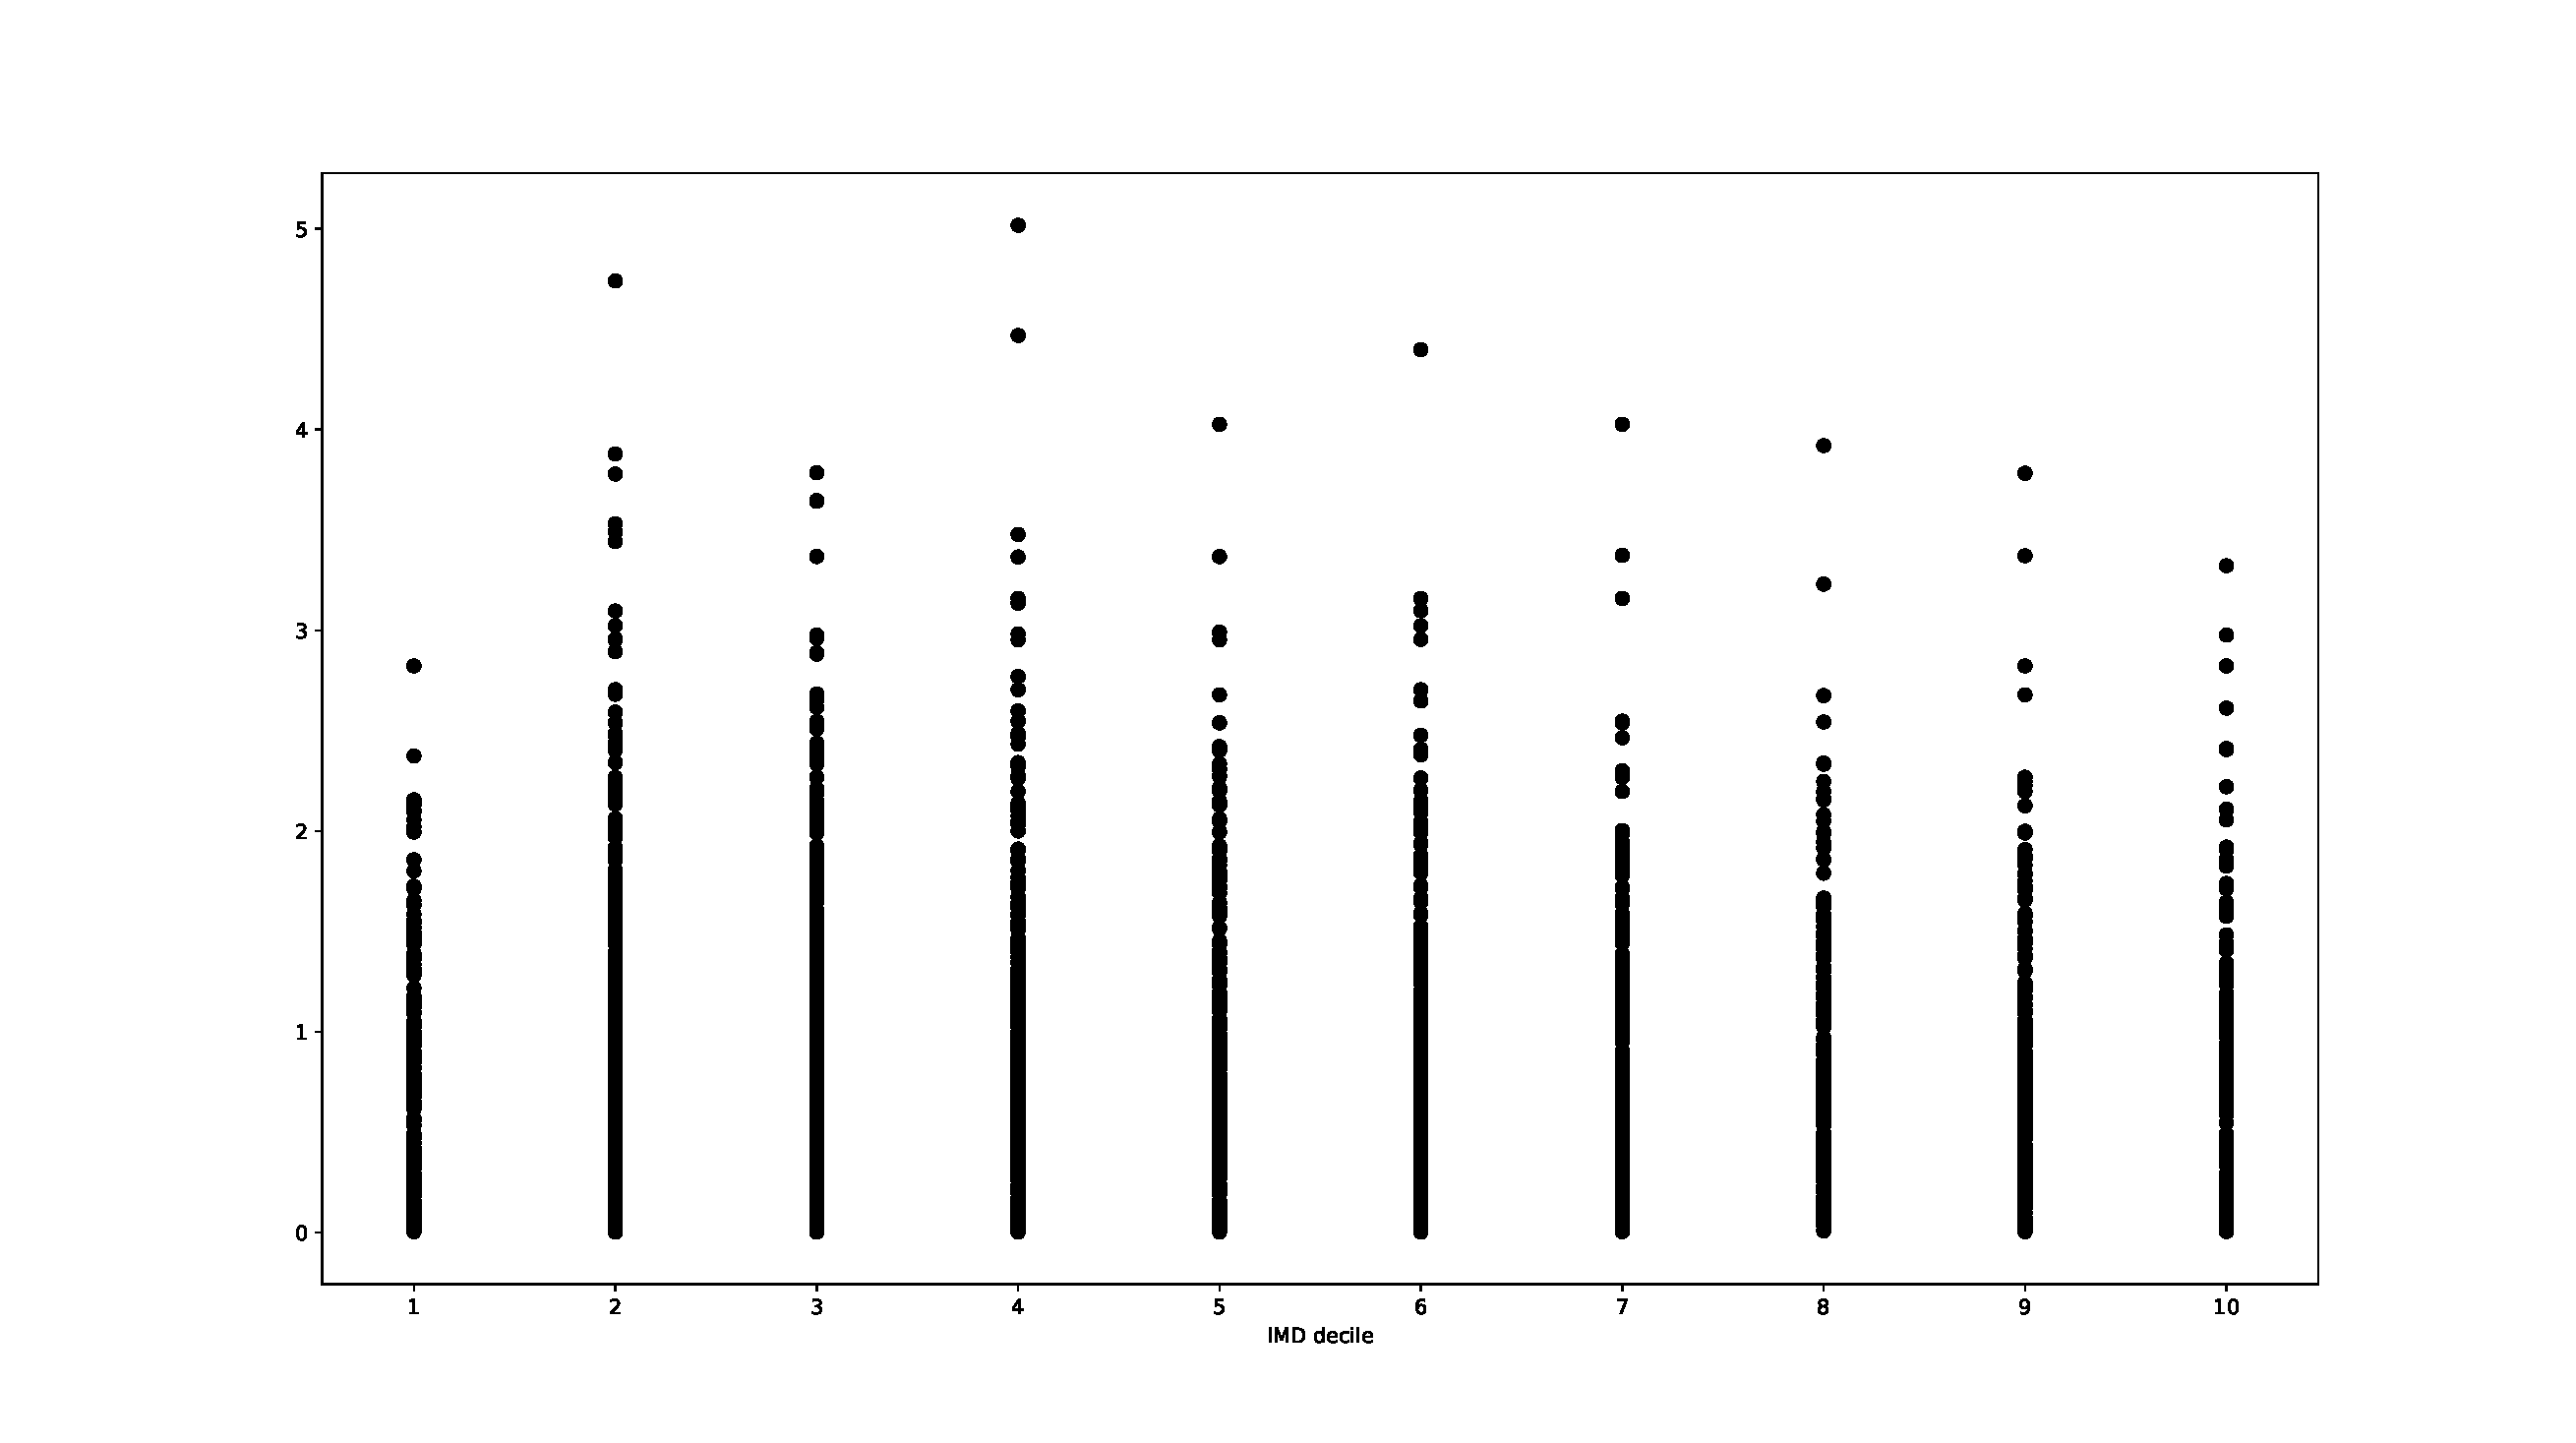
\includegraphics[width=\linewidth,keepaspectratio]{spatial_algorithms/scatter_plot.pdf}
		\caption{Scatter plot}
	\end{subfigure}
	\begin{subfigure}[b]{0.45	\linewidth}
		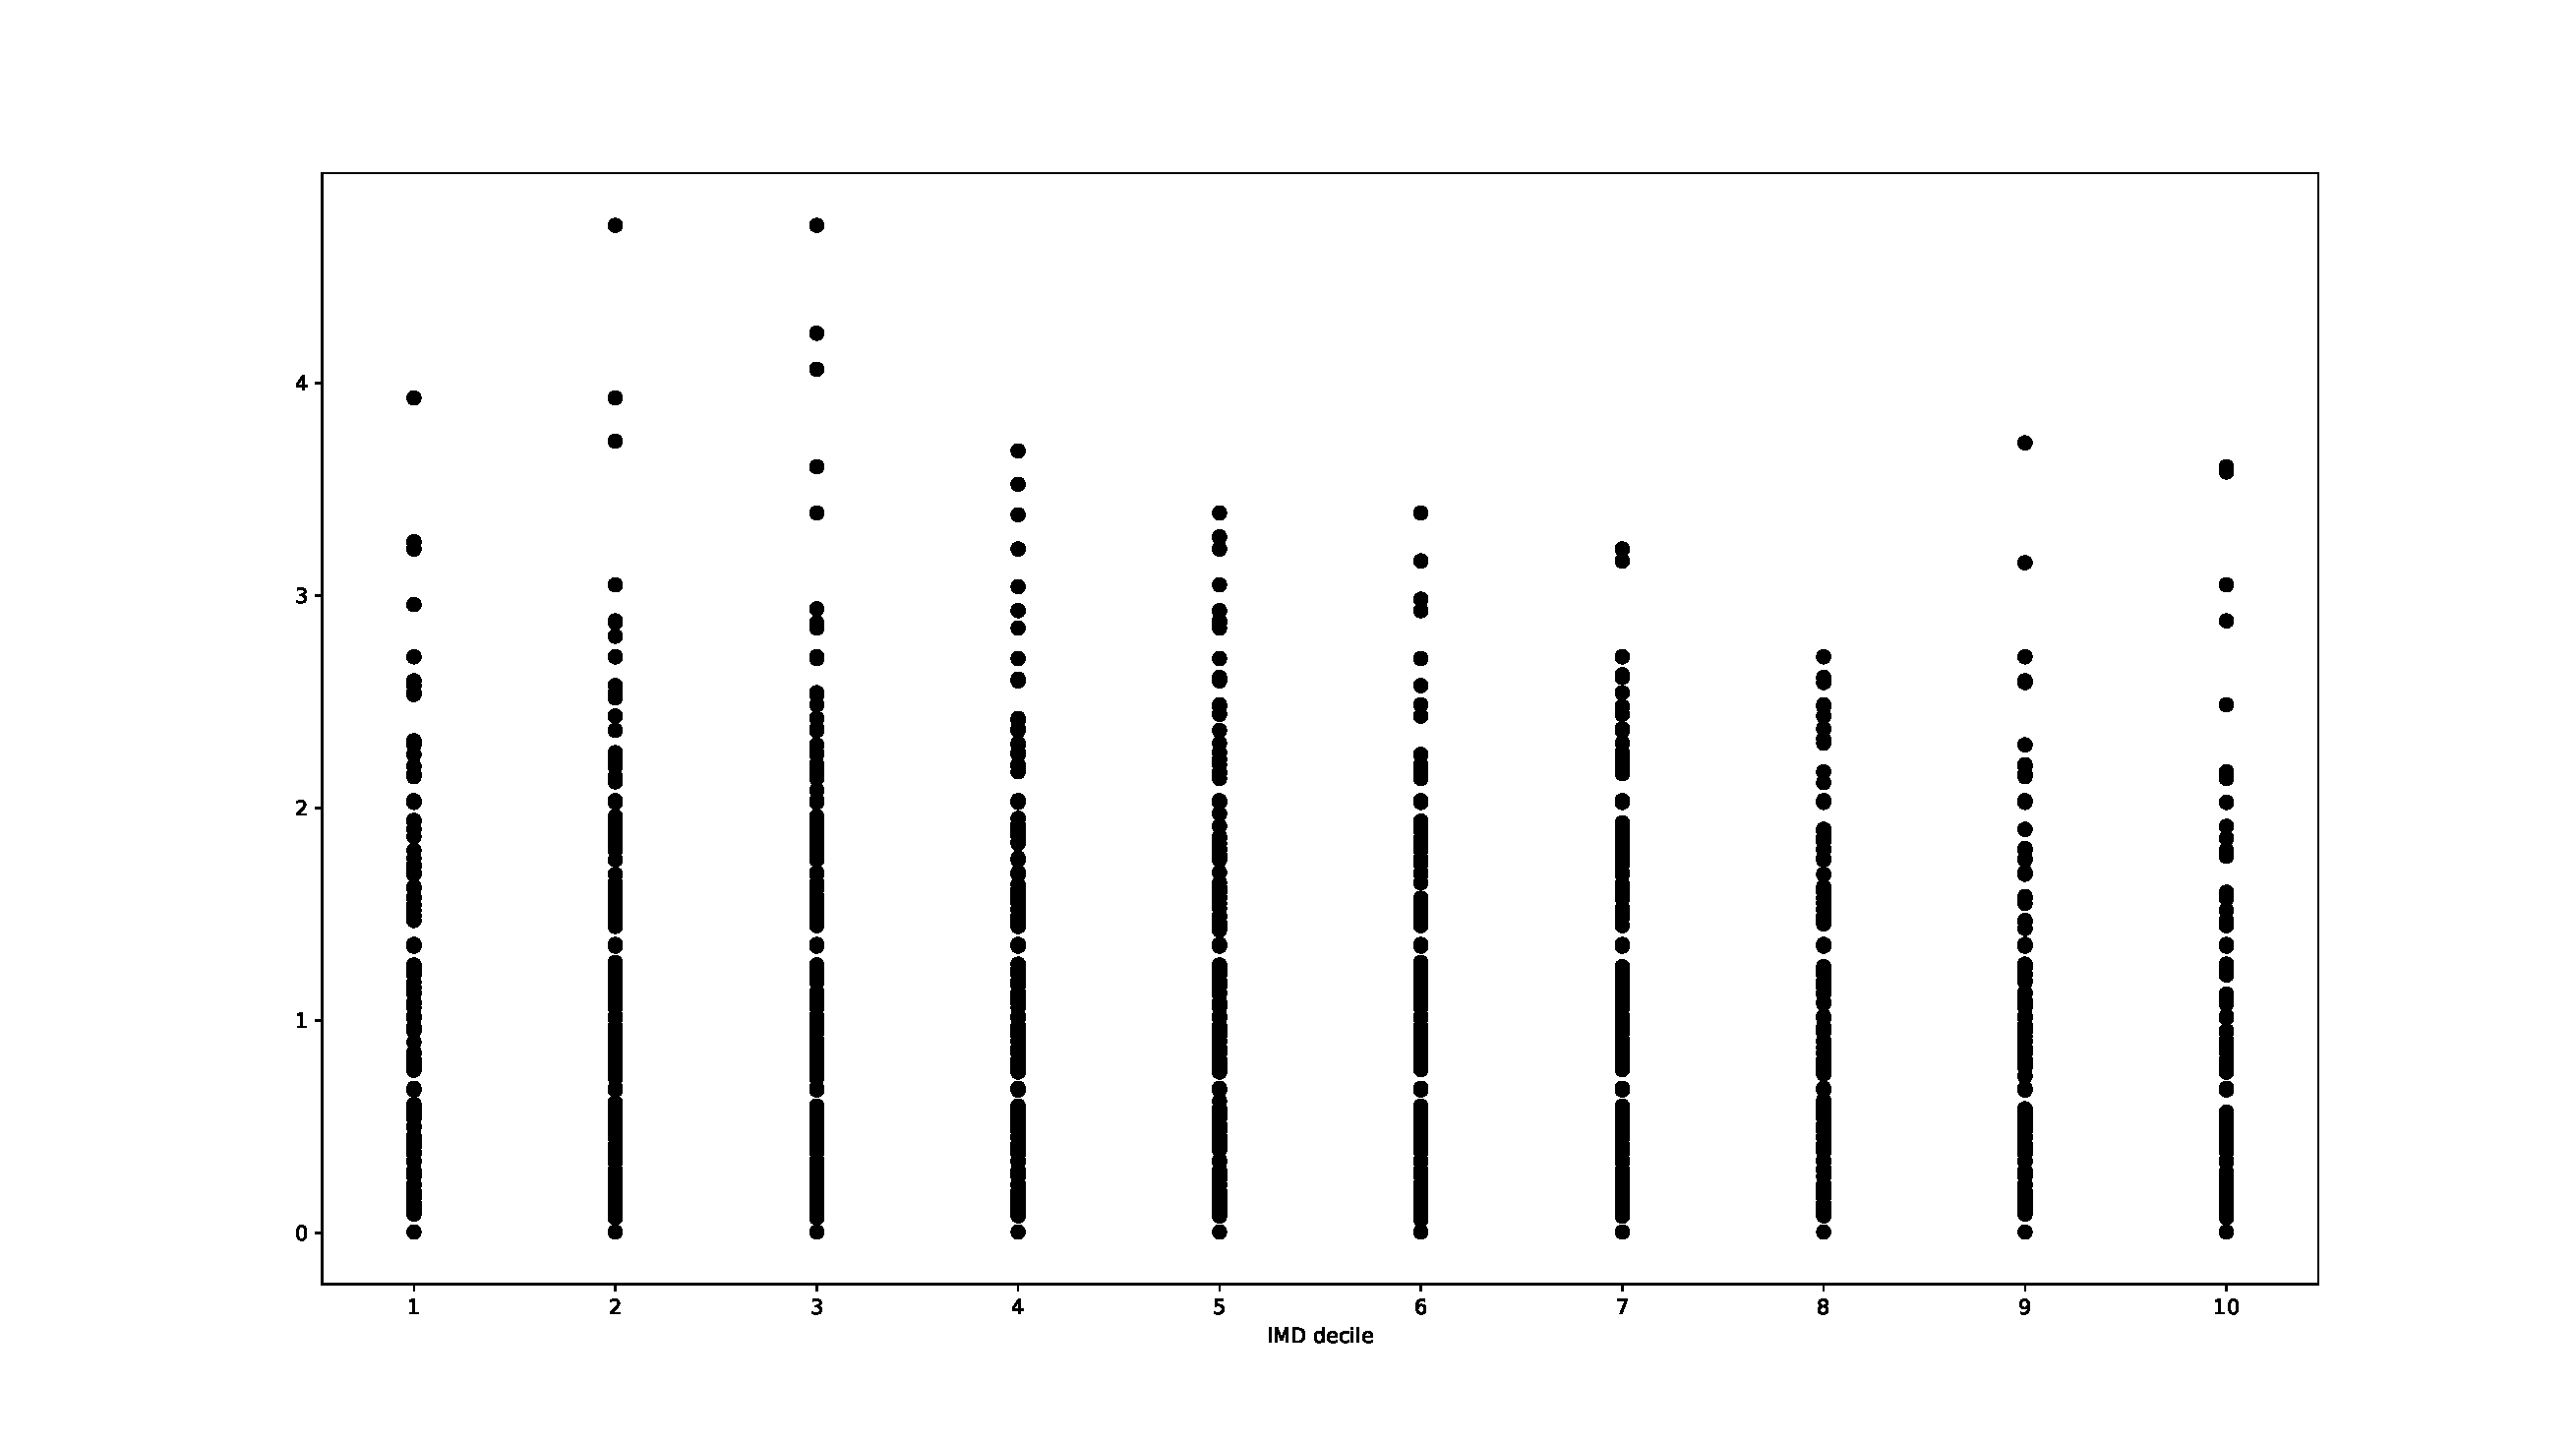
\includegraphics[width=\linewidth,keepaspectratio]{spatial_algorithms/ztest.pdf}
		\caption{Z-test}
	\end{subfigure}	
\caption{\textit{IMD spatial outliers}}
\label{fig:IMD_spatial_outliers}
\end{figure}

\section{Conclusion and future work}
[TBD]

%\begin{thebibliography}{10}
%\end{thebibliography}
\end{document}


